\documentclass[12pt,a4paper,twoside]{report}
% -------------------------------------------------------------------- %
% Pacotes

\usepackage[utf8]{inputenc}
\usepackage[T1]{fontenc}
\usepackage[brazil]{babel}
\usepackage[fixlanguage]{babelbib}
\usepackage[pdftex]{graphicx}      % usamos arquivos pdf/png como figuras
\usepackage{setspace}              % espaçamento flexvel
\usepackage{indentfirst}           % indentação do primeiro parágrafo
\usepackage{makeidx}               % índice remissivo
\usepackage[nottoc]{tocbibind}     % acrescentamos a bibliografia/indice/conteudo no Table of Contents
\usepackage{courier}               % usa o Adobe Courier no lugar de Computer Modern Typewriter
\usepackage{type1cm}               % fontes realmente escaláveis
\usepackage{titletoc}
\usepackage{ucs}
\usepackage[font=small,format=plain,labelfont=bf,up,textfont=it,up]{caption}
\usepackage[usenames,svgnames,dvipsnames]{xcolor}
\usepackage[a4paper,top=2.54cm,bottom=2.0cm,left=2.0cm,right=2.54cm]{geometry} % margens
\usepackage{amsmath} 

\usepackage[pdftex,plainpages=false,pdfpagelabels,pagebackref,colorlinks=true,citecolor=DarkGreen,
linkcolor=NavyBlue,urlcolor=DarkRed,filecolor=green,bookmarksopen=true]{hyperref} % links coloridos
\usepackage[all]{hypcap}                % soluciona o problema com o hyperref e capítulos
\usepackage[square,sort,nonamebreak,comma]{natbib}  % citação bibliográfica alpha
\fontsize{60}{62}\usefont{OT1}{cmr}{m}{n}{\selectfont}
\usepackage{upquote}                    % formata apóstrofes '
\usepackage{textcomp}

% Para formatar corretamente as URLs
\usepackage{url}
% -------------------------------------------------------------------- %
% Cabeçalhos similares ao TAOCP de Donald E. Knuth
\usepackage{fancyhdr}
\pagestyle{fancy}
\fancyhf{}
\renewcommand{\chaptermark}[1]{\markboth{\MakeUppercase{#1}}{}}
\renewcommand{\sectionmark}[1]{\markright{\MakeUppercase{#1}}{}}
\renewcommand{\headrulewidth}{0pt}

% -------------------------------------------------------------------- %
\graphicspath{{./imagens/}}        % caminho das figuras
\frenchspacing                     % arruma o espaço: id est (i.e.) e exempli gratia (e.g.)
\urlstyle{same}                    % URL com o mesmo estilo do texto e no mono-spaced
\makeindex                         % para o índice remissivo
\raggedbottom                      % para no permitir espaços extras no texto
\fontsize{60}{62}\usefont{OT1}{cmr}{m}{n}{\selectfont}
\cleardoublepage
\normalsize

% -------------------------------------------------------------------- %
% Cores para formatação de código
\usepackage{color}
\definecolor{vermelho}{rgb}{0.6,0,0} % para strings
\definecolor{verde}{rgb}{0.25,0.5,0.35} % para comentários
\definecolor{roxo}{rgb}{0.5,0,0.35} % para palavras-chaves
\definecolor{azul}{rgb}{0.25,0.35,0.75} % para strings
\definecolor{cinza-claro}{gray}{0.95}
% -------------------------------------------------------------------- %
% Opções de listagem usados para o código fonte
% Ref: http://en.wikibooks.org/wiki/LaTeX/Packages/Listings



\usepackage{listings}           % para formatar código-fonte (ex. em Java)
\usepackage{xcolor} 

\lstset{ %
language=[Objective]Caml,  % seleciona a linguagem do código (aqui em lstlang0.sty
basicstyle=\footnotesize\ttfamily, % o tamanho da fonte usado no código
commentstyle=\color{verde}\bfseries,  % formatação de comentários
stringstyle=\color{azul},    % formatação de strings
upquote=true,
numbers=left,                   % onde colocar os números de linha
numberstyle=\tiny,  % o tamanho da fonte usada para a numeração das linhas
stepnumber=1,                   % o intervalo entre dois números de linhas. Se for 1, numera cada uma.
numbersep=5pt,                  % how far the line-numbers are from the code
showspaces=false,               % show spaces adding particular underscores
showstringspaces=false,         % underline spaces within strings
showtabs=false,                 % show tabs within strings adding particular underscores
keywordstyle=\color{roxo}\bfseries,
keywordstyle=[1]\color{roxo}\bfseries,
keywordstyle=[2]\color{verde}\bfseries,
%        keywordstyle=[3]\textbf,    %
%        keywordstyle=[4]\textbf,   \sqrt{\sqrt{}} %
frame=b,                   % adds a frame around the code
framerule=0.6pt,
tabsize=2,                      % sets default tabsize to 2 spaces
captionpos=t,                   % sets the caption-position to top
breaklines=true,                % sets automatic line breaking
breakatwhitespace=false,        % sets if automatic breaks should only happen at whitespace
escapeinside={\%*}{*)},         % if you want to add a comment within your code
backgroundcolor=\color[rgb]{1.0,1.0,1.0}, % choose the background color.
rulecolor=\color[rgb]{0.8,0.8,0.8},
extendedchars=true,
xleftmargin=10pt,
xrightmargin=10pt,
framexleftmargin=10pt,
framexrightmargin=10pt,
literate={â}{{\^{a}}}1  % para formatar corretamente os acentos do Português ao usar utf8
    {ê}{{\^{e}}}1
    {ô}{{\^{o}}}1  
    {Â}{{\^{A}}}1
    {Ê}{{\^{E}}}1
    {Ô}{{\^{O}}}1
    {á}{{\'{a}}}1
    {é}{{\'{e}}}1
    {í}{{\'{i}}}1
    {ó}{{\'{o}}}1
    {ú}{{\'{u}}}1
    {Á}{{\'{A}}}1
    {É}{{\'{E}}}1
    {Í}{{\'{I}}}1
    {Ó}{{\'{O}}}1
    {Ú}{{\'{U}}}1
    {à}{{\`{a}}}1
    {À}{{\`{A}}}1
    {ã}{{\~{a}}}1
    {õ}{{\~{o}}}1
    {Ã}{{\~{A}}}1
    {Õ}{{\~{O}}}1
    {ç}{{\c{c}}}1
    {Ç}{{\c{C}}}1
    {ü}{{\"u}}1
    {Ü}{{\"U}}1
}

\renewcommand{\lstlistingname}{Listagem}
\renewcommand{\lstlistlistingname}{Lista de Listagens}

% Definição de novos estilos
\lstdefinestyle{Bash}
    {language=bash,frame=single,numbers=none,basicstyle=\footnotesize\ttfamily,
     morekeywords={cp,mkdir,sudo,tar}}

% Definição de novos ambientes
\lstnewenvironment{terminal}
  {\lstset{style=Bash}}
  {}

\lstnewenvironment{ocaml}
  {\lstset{basicstyle=\scriptsize\ttfamily,
           frame=single,
           frameround=tttt,
           framerule=2pt,
           numbers=none,
           rulecolor=\color{Salmon}}}
  {}

\lstnewenvironment{xml}
   {\lstset{language=XML,frame=single,numbers=none}}
   {}

\lstnewenvironment{interprete}
  {\lstset{frame=single,
            frameround=tttt,
            numbers=none,
            basicstyle=\ttfamily,
            framerule=2pt,
            rulecolor=\color{CadetBlue}}}
  {}
% Formata o caption da listagem
% \DeclareCaptionFont{blue}{\color{blue}} 

% \captionsetup[lstlisting]{singlelinecheck=false, labelfont={blue}, textfont={blue}}
\usepackage{caption}
\DeclareCaptionFont{white}{\color{white}}
\DeclareCaptionFormat{listing}{\colorbox[cmyk]{0.43, 0.35, 0.35,0.01}{\parbox{\textwidth}{\hspace{15pt}#1#2#3}}}
\captionsetup[lstlisting]{format=listing,labelfont=white,textfont=white, singlelinecheck=false, margin=0pt, font={bf,footnotesize}}

\newcommand{\ListingsPath}{./codigos}
% Inclui o nome do arquivo como Caption 
\newcommand{\filelisting}[2][]{%
    \lstinputlisting[caption={\texttt{\detokenize{#2}}},#1]{\ListingsPath/#2}%
}

% ---------------------------------------------------------------------------- %

% ---------------------------------------------------------------------------- %

\title{Construção de Compiladores - Java para JVM}
\date{19/3/2018}
\author{  \\
\textbf{Nome:} Gustavo Miranda de Aguiar \\
\textbf{Matrícula:} 11421BCC021 \\
\textbf{Email:} \texttt{\small \url{gumiranda@ufu.br }}\\
\textbf{Profº.:} Alexsandro Santos Soares
\vspace{1cm} \\
Faculdade de Computação \\
Universidade Federal de Uberlândia
}
\date{\today}

%\includeonly{cap-clojure,magical,short}
\begin{document}
  \maketitle
% -------------------------------------------------------------------- %
% Listas de figuras, tabelas e códigos criadas automaticamente       
% -------------------------------------------------------------------- %

% -------------------------------------------------------------------- %
% Sumário
\tableofcontents    

% Capítulos do trabalho

% cabeçalho para as páginas de todos os capítulos
\fancyhead[RE,LO]{\thesection}

%\singlespacing              % espaçamento simples
\setlength{\parskip}{0.15in} % espaçamento entre paragráfos
\chapter{Introdução}
Esse relatório tem como objetivo apresentar as tecnologias utilizadas para a construção de um compilador para a linguagem Java(MiniJava) utilizando a JVM (Máquina Virtual do Java) .
O sistema operacional a ser utilizado é o Ubuntu 14.04 e a linguagem do desenvolvimento do compilador será Ocaml.
\section{Preparando o ambiente}
Neste primeiro capítulo vamos aprender a preparar o ambiente para que possamos desenvolver
nosso compilador de MiniJava para JVM.
\subsection{Instalação do JDK}
Após a instalação do Ubuntu , será efetuada a instalação do JDK com os seguintes comandos no terminal. 


\begin{terminal}
> sudo add-apt-repository ppa:webupd8team/java
\end{terminal}


\begin{terminal}
> sudo apt-get update
\end{terminal}


\begin{terminal}
> sudo apt-get install oracle-java7-installer
\end{terminal}

\subsection{OCaml}

           Ocaml é a linguagem de programação escolhida para a implementação do compilador. Para instalar a Ocaml no Ubuntu utiliza-se o seguinte comando:

         \begin{terminal}
         > sudo apt-get install ocaml
         \end{terminal}

\subsection{Instalação do Jasmin}
O Jasmin será responsável pela conversão de um programa com sintaxe que usa instruções da JVM em um arquivo binário.
Entramos em \url{http://jasmin.sourceforge.net/} e fazemos o download do arquivo.Em seguida descompactamos o arquivo e copiamos o arquivo "jasmin.jar" para a mesma pasta que contém os arquivos a serem compilados por ele.



\chapter{JVM}
Neste capítulo aprofundamos as características da Java Virtual Machine.
\section{O que é JVM?}
JVM basicamente é um processador virtual responsável por carregar e executar as aplicações Java, realizando a conversão de bytecodes em código de máquina. 

A JVM é uma máquina de pilha, ou seja suas instruções utilizam a
pilha para armazenar resultados intermediários, ao invés de utilizar registradores como é feito em
arquiteturas concretas. Isto permite a definição de um conjunto mais simples de instruções que é
facilmente implementado em diferentes arquiteturas.
Um ponto importante a ser ressaltado é o fato de que a JVM não conhece nada da
linguagem Java. Ela apenas entende  os arquivos .class gerados a partir dos arquivos .java. Portanto
a JVM permite rodar outras linguagens desde que elas sejam traduzidas para .class como Haskell, Pascal, Ada, Scala.[2]
\section{Estrutura da JVM}
Na estrutrura temos:


\begin{figure}[!ht]
\centering
\caption{Uma JVM implementada em software no topo de um sistema operacional
hospedeiro.
      \label{fig:2}}
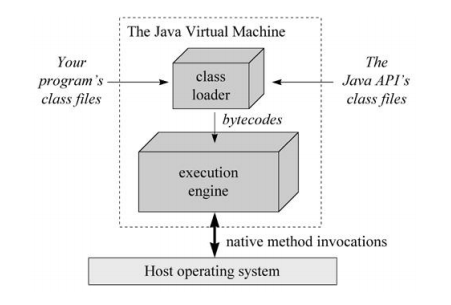
\includegraphics[scale=1]{imagens/jvm.png}
\end{figure}
 A \textbf{ Class loader} é a responsável por carregar os arquivos das classes do programa e da API
do Java, além de verificar a corretude das classes, inicializar a memória para as
variáveis de classe e ajudar na resolução de símbolos. [3]

\textbf{Execution engine} é onde os bytecodes são executados,e onde temos mais implementações
diferentes na JVM. [3]

\textbf{Native method invocations} é  o que faz a interação com o Sistema Operacional (SO),
onde se tem a ligação entre o JVM e o SO. Os métodos nativos geralmente são
escritos em C e C++. [3]

\section{Tipos de Dados do JVM}
No JVM existem tipos primitivos de dados, tais como byte, short, int, long, float, double e
referencias a objetos, etc... O tamanho de uma palavra(“word”) no JVM vária de acordo com a
implementação e deve ser grande o suficiente para armazenar os tipos primitivos supracitados, em
exceção ao long e double, que por sua vez duas words devem ser capazes de armazená-los.
Os tipos numéricos são subdivididos em tipos inteiros e em pontos flutuantes, como pode ser
visto abaixo:[3]\\
• byte - 9 bits com sinal\\
• char - 16 bits sem sinal\\
• short - 16 bits com sinal\\
• int - 32 bits com sinal\\
• long - 64 bits com sinal\\
• float - 32 bits com sinal\\
• double - 64 bits com sinal\\
\section{Instruções da JVM}
Uma instrução da JVM consiste de um opcode de um byte e pode ter argumentos e dados
que serão usandos na operação. A opção de ter a instrução em apenas um byte permite maior
simplicidade e limita o número de instruções.
O opcode mnemônico na maioria das instruções representa o tipo sobre qual ela opera. Possui
uma letra para representar cada tipo:[3]
• i: para int;\\
• l: para long;\\
• s: para short;\\
• b: para byte;\\
• c: para char;\\
• f: para float;\\
• d: para double;\\
• a: para uma referência;
\chapter{Jasmin}
Neste capítulo aprofundamos as características do Jasmin.
\section{O que é Jasmin?}
 Jasmin é um assembler para Java Virtual Machine(JVM).A função dele é converter códigos escritos seguindo uma sintaxe assembler - que utiliza o conjunto de instruções da JVM - em códigos binários de classes Java adequados para serem carregados por um sistema Java Runtime. Resumindo, o Jasmin recebe um arquivo .j e produz um arquivo .class .\\
Sempre que possivel, o Jasmin adota um mapeamento   \texttt{one-to-one} entre sua sintaxe e as convenções seguidas pelos arquivos de classe Java.Por exemplo,os nomes dos pacotes em Jasmin são delimitados com o caractere   "\texttt{/}"  (por exemplo," \texttt{java/lang/String}" usado pelo formato de arquivo da classe,em vez do caractere   "\texttt{.}" (  \texttt{"java.lang.String"} )  usado na linguagem Java.\\ Usando o Jasmin,é possível experimentar quase todos os recursos da JVM,incluindo métodos,campos,sub-rotinas, \texttt{exception handlers},etc.
\section{Como executar o Jasmin?}
O arquivo jasmin.jar é um arquivo JAR executável que executa o Jasmin. Por exemplo:
\begin{terminal}
>   java -jar jasmin.jar nomedoarquivodesaida.j 
\end{terminal}
O Jasmin analisa a diretriz .class contida no arquivo nomedoarquivodesaida.j  para decidir onde colocar o arquivo de classe de saída. Então, se nomedoarquivodesaida.j  começar com:     ".class pacoteexemplo/MinhaClasse"
então Jasmin colocará o arquivo de classe de saída "MinhaClasse.class" no subdiretório "pacoteexemplo" do diretório atual. Ele criará o diretório pacoteexemplo se ele não existir.
Podemos  usar a opção "-d" para dizer ao jasmin que coloque a saída em um diretório alternativo. Por exemplo,
\begin{terminal}
>   java -jar jasmin.jar -d / tmp nomedoarquivodesaida.j 
\end{terminal}
Dessa forma a saída será gerada em /tmp/pacoteexemplo/MinhaClasse.class.


\section{Assembly Jasmin}
Jasmin usa o padrão para a JVM mnemônico (parâmetros) opcodes como instrução de nomes.
Os arquivos para Jasmin começam com as informações sobre a classe a ser definida no arquivo
- como o nome de classe, o nome do arquivo fonte que originou a partir da classe,o nome da
superclasse, etc.
 \textit{.font/opcional .class .super}

 O método (função) começa com  \textit{ .method} e termina com   \textit{ .end
method}. No método principal utiliza-se \textit{ .limit stack 5}
 (configura o tamanho da pilha para o método
principal (main) operando a 5) e  \textit{ .limit locals 100}
 (define o número de variáveis locais do método
principal (main) para 100).
Abaixo estão relatadas mais algumas instruções utilizadas no Jasmin:[3]\\ \\
 \textbf{iload} carrega o valor de uma variável local que é um inteiro para o topo da pilha.\\
 \textbf{istore} carrega o valor do topo da pilha para a variável.\\
 \textbf{fload} carrega o valor de uma variável local que é um float para o topo da pilha.\\
 \textbf{fstore} carrega o valor do topo da pilha que é um float para a variável.\\
 \textbf{ldc} desempilha a constante da pilha.\\
 \textbf{dup} a palavra no topo da pilha é duplicado.\\
 \textbf{pop} retira o valor que esta no topo da pilha.\\
 \textbf{swap} troca dois operandos da pilha (uma troca, o primeiro vira o segundo e o segundo vira o primeiro).\\
 \textbf{iadd} adiciona dois inteiros.\\
 \textbf{idiv} divide dois inteiros.\\
 \textbf{imul}  multiplica dois inteiros.\\
 \textbf{isub} subtrai dois inteiros.\\
 \textbf{fadd} adiciona dois float.\\
 \textbf{fdiv} divide dois float.\\
 \textbf{fmul} multiplica dois float.\\
 \textbf{fsub} subtrai dois float.\\
 \textbf{goto}  ir para o marcador.\\
 \textbf{ifeq} ir para o rótulo (marcador), se o valor no topo da pilha é 0.\\
 \textbf{ifge} ir para o rótulo, se o valor no topo da pilha é igual ou superior (maior) a 0.\\
 \textbf{ifgt} ir para o rótulo, se o valor no topo da pilha é superior (maior) a 0.\\
 \textbf{ifle} ir para o rótulo, se o valor no topo da pilha é inferior (menor) ou igual a 0.\\
 \textbf{iflt}ir para o rótulo, se o valor no topo da pilha é inferior (menor) a 0.\\
 \textbf{ifne} ir para o rótulo, se o valor no topo da pilha não é igual a 0.\\
 \textbf{iand} AND (inteiros).\\
 \textbf{ior } OR (inteiros).\\
 \textbf{ i2f} converte inteiro para float.\\
 \textbf{ f2i} converte float para inteiro.\\
 \textbf{ jsr} retorna o endereço da pilha e "pula"para subrotina indicada.\\
 \textbf{ ret} retorna o endereço da subrotina que esta armazenado a variável local.\\
 \textbf{ invokevirtual} é a forma padrão para a chamada de um método.\\ \\
Existem várias outras instruções como exemplo de mais algumas são: bipush, sipush, iinc, ifnull,
anewarray, checkcast, instanceof, new, getfeld, getstatic, putfeld, putstatic, newarray, iconst, entre outros.\\

\chapter{Exemplos de programas escritos em Java \label{ap:Testes}}
\section{Conversão para JAVA}
Todos os códigos Java foram gerados pelo javac com o seguinte  comando: 
\begin{terminal}
> javac nome.java
\end{terminal}


\section{Nano1.java}
\lstinputlisting[label={arq:Nano1.java}, language=Java,
caption={Nano1.java}]{codigos/MiniJava/Nano1.java}
\section{Nano2.java}
\lstinputlisting[label={arq:Nano2.java}, language=Java,
caption={Nano2.java}]{codigos/MiniJava/Nano2.java}
\section{Nano3.java}
\lstinputlisting[label={arq:Nano3.java}, language=Java,
caption={Nano3.java}]{codigos/MiniJava/Nano3.java}
\section{Nano4.java}
\lstinputlisting[label={arq:Nano4.java}, language=Java,
caption={Nano4.java}]{codigos/MiniJava/Nano4.java}
\section{Nano5.java}
\lstinputlisting[label={arq:Nano5.java}, language=Java,
caption={Nano5.java}]{codigos/MiniJava/Nano5.java}
\section{Nano6.java}
\lstinputlisting[label={arq:Nano6.java}, language=Java,
caption={Nano6.java}]{codigos/MiniJava/Nano6.java}
\section{Nano7.java}
\lstinputlisting[label={arq:Nano7.java}, language=Java,
caption={Nano7.java}]{codigos/MiniJava/Nano7.java}
\section{Nano8.java}
\lstinputlisting[label={arq:Nano8.java}, language=Java,
caption={Nano8.java}]{codigos/MiniJava/Nano8.java}
\section{Nano9.java}
\lstinputlisting[label={arq:Nano9.java}, language=Java,
caption={Nano9.java}]{codigos/MiniJava/Nano9.java}
\section{Nano10.java}
\lstinputlisting[label={arq:Nano10.java}, language=Java,
caption={Nano10.java}]{codigos/MiniJava/Nano10.java}
\section{Nano11.java}
\lstinputlisting[label={arq:Nano11.java}, language=Java,
caption={Nano11.java}]{codigos/MiniJava/Nano11.java}
\section{Nano12.java}
\lstinputlisting[label={arq:Nano12.java}, language=Java,
caption={Nano12.java}]{codigos/MiniJava/Nano12.java}

\section{Micro1.java}
\lstinputlisting[label={arq:Micro1.java}, language=Java,
caption={Micro1.java}]{codigos/MiniJava/Micro1.java}
\section{Micro2.java}
\lstinputlisting[label={arq:Micro2.java}, language=Java,
caption={Micro2.java}]{codigos/MiniJava/Micro2.java}
\section{Micro3.java}
\lstinputlisting[label={arq:Micro3.java}, language=Java,
caption={Micro3.java}]{codigos/MiniJava/Micro3.java}
\section{Micro4.java}
\lstinputlisting[label={arq:Micro4.java}, language=Java,
caption={Micro4.java}]{codigos/MiniJava/Micro4.java}
\section{Micro5.java}
\lstinputlisting[label={arq:Micro5.java}, language=Java,
caption={Micro5.java}]{codigos/MiniJava/Micro5.java}
\section{Micro6.java}
\lstinputlisting[label={arq:Micro6.java}, language=Java,
caption={Micro6.java}]{codigos/MiniJava/Micro6.java}
\section{Micro7.java}
\lstinputlisting[label={arq:Micro7.java}, language=Java,
caption={Micro7.java}]{codigos/MiniJava/Micro7.java}
\section{Micro8.java}
\lstinputlisting[label={arq:Micro8.java}, language=Java,
caption={Micro8.java}]{codigos/MiniJava/Micro8.java}
\section{Micro9.java}
\lstinputlisting[label={arq:Micro9.java}, language=Java,
caption={Micro9.java}]{codigos/MiniJava/Micro9.java}
\section{Micro10.java}
\lstinputlisting[label={arq:Micro10.java}, language=Java,
caption={Micro10.java}]{codigos/MiniJava/Micro10.java}
\section{Micro11.java}
\lstinputlisting[label={arq:Micro11.java}, language=Java,
caption={Micro11.java}]{codigos/MiniJava/Micro11.java}


\chapter{Exemplos de programas escritos em Java convertidos para Assembly \label{ap:Testes}}
\section{Conversão para Assembly}
Todos os codigos Java para Assembly foram convertidos usando o comando javap da seguinte forma:
\begin{terminal}
javap -c nome.class
\end{terminal} 
Depois disso modificamos a saída desse comando para um arquivo Jasmin válido (um arquivo .j) .
\section{NanoPrograma1}
\begin{terminal}
.class public Nano1
.super java/lang/Object

.method public <init>()V
  .limit stack 1
  .limit locals 1
  .line 2
  0: aload_0
  1: invokespecial java/lang/Object/<init>()V
  4: return
.end method

.method public static main([Ljava/lang/String;)V
  .limit stack 0
  .limit locals 1
  .line 4
  0: return
.end method

\end{terminal}

\section{NanoPrograma2}
\begin{terminal}
.class public Nano2
.super java/lang/Object

.method public <init>()V
  .limit stack 1
  .limit locals 1
  .line 3
  0: aload_0
  1: invokespecial java/lang/Object/<init>()V
  4: return
.end method

.method public static main([Ljava/lang/String;)V
  .limit stack 0
  .limit locals 2
  .line 6
  0: return
.end method

\end{terminal}\section{NanoPrograma3}
\begin{terminal}
.class public Nano3
.super java/lang/Object

.method public <init>()V
  .limit stack 1
  .limit locals 1
  .line 3
  0: aload_0
  1: invokespecial java/lang/Object/<init>()V
  4: return
.end method

.method public static main([Ljava/lang/String;)V
  .limit stack 1
  .limit locals 2
  .line 6
  0: iconst_1
  1: istore_1
  .line 7
  2: return
.end method
\end{terminal}\section{NanoPrograma4}
\begin{terminal}
.class public Nano4
.super java/lang/Object

.method public <init>()V
  .limit stack 1
  .limit locals 1
  .line 3
  0: aload_0
  1: invokespecial java/lang/Object/<init>()V
  4: return
.end method

.method public static main([Ljava/lang/String;)V
  .limit stack 1
  .limit locals 2
  .line 6
  0: iconst_3
  1: istore_1
  .line 7
  2: return
.end method
\end{terminal}\section{NanoPrograma5}
\begin{terminal}
.class public Nano5
.super java/lang/Object

.method public <init>()V
  .limit stack 1
  .limit locals 1
  .line 3
  0: aload_0
  1: invokespecial java/lang/Object/<init>()V
  4: return
.end method

.method public static main([Ljava/lang/String;)V
  .limit stack 2
  .limit locals 2
  .line 6
  0: iconst_2
  1: istore_1
  .line 7
  2: getstatic java/lang/System/out Ljava/io/PrintStream;
  5: iload_1
  6: invokevirtual java/io/PrintStream/print(I)V
  .line 8
  9: return
.end method

\end{terminal}\section{NanoPrograma6}
\begin{terminal}
.class public Nano6
.super java/lang/Object

.method public <init>()V
  .limit stack 1
  .limit locals 1
  .line 3
  0: aload_0
  1: invokespecial java/lang/Object/<init>()V
  4: return
.end method

.method public static main([Ljava/lang/String;)V
  .limit stack 2
  .limit locals 2
  .line 6
  0: iconst_m1
  1: istore_1
  .line 7
  2: getstatic java/lang/System/out Ljava/io/PrintStream;
  5: iload_1
  6: invokevirtual java/io/PrintStream/print(I)V
  .line 9
  9: return
.end method
\end{terminal}\section{NanoPrograma7}
\begin{terminal}
.class public Nano7
.super java/lang/Object

.method public <init>()V
  .limit stack 1
  .limit locals 1
  .line 3
  0: aload_0
  1: invokespecial java/lang/Object/<init>()V
  4: return
.end method

.method public static main([Ljava/lang/String;)V
  .limit stack 2
  .limit locals 2
  .line 6
  0: iconst_1
  1: istore_1
  .line 7
  2: iload_1
  3: iconst_1
  4: if_icmpne Label14
  .line 8
  7: getstatic java/lang/System/out Ljava/io/PrintStream;
  10: iload_1
  11: invokevirtual java/io/PrintStream/print(I)V
Label14:
  .line 10
  14: return
  ; append_frame (frameNumber = 0)
  ; frame_type = 252, offset_delta = 14
  ; frame bytes: 252 0 14 1
  .stack
    offset 14
    locals Integer
    .end stack
.end method

\end{terminal}\section{NanoPrograma8}
\begin{terminal}
.class public Nano8
.super java/lang/Object

.method public <init>()V
  .limit stack 1
  .limit locals 1
  .line 3
  0: aload_0
  1: invokespecial java/lang/Object/<init>()V
  4: return
.end method

.method public static main([Ljava/lang/String;)V
  .limit stack 2
  .limit locals 2
  .line 6
  0: iconst_1
  1: istore_1
  .line 7
  2: iload_1
  3: iconst_1
  4: if_icmpne Label17
  .line 8
  7: getstatic java/lang/System/out Ljava/io/PrintStream;
  10: iload_1
  11: invokevirtual java/io/PrintStream/print(I)V
  14: goto Label25
Label17:
  .line 11
  17: getstatic java/lang/System/out Ljava/io/PrintStream;
  20: ldc "0"
  22: invokevirtual java/io/PrintStream/print(Ljava/lang/String;)V
Label25:
  .line 14
  25: return
  ; append_frame (frameNumber = 0)
  ; frame_type = 252, offset_delta = 17
  ; frame bytes: 252 0 17 1
  .stack
    offset 17
    locals Integer
    .end stack
  ; same_frame (frameNumber = 1)
  ; frame_type = 7, offset_delta = 7
  ; frame bytes: 7
  .stack
    offset 25
    locals Integer
    .end stack
.end method
\end{terminal}\section{NanoPrograma9}
\begin{terminal}
.class public Nano9
.super java/lang/Object

.method public <init>()V
  .limit stack 1
  .limit locals 1
  .line 3
  0: aload_0
  1: invokespecial java/lang/Object/<init>()V
  4: return
.end method

.method public static main([Ljava/lang/String;)V
  .limit stack 2
  .limit locals 2
  .line 6
  0: iconst_1
  1: istore_1
  .line 7
  2: iload_1
  3: iconst_1
  4: if_icmpne Label17
  .line 8
  7: getstatic java/lang/System/out Ljava/io/PrintStream;
  10: iload_1
  11: invokevirtual java/io/PrintStream/print(I)V
  14: goto Label25
Label17:
  .line 10
  17: getstatic java/lang/System/out Ljava/io/PrintStream;
  20: ldc "0"
  22: invokevirtual java/io/PrintStream/print(Ljava/lang/String;)V
Label25:
  .line 13
  25: return
  ; append_frame (frameNumber = 0)
  ; frame_type = 252, offset_delta = 17
  ; frame bytes: 252 0 17 1
  .stack
    offset 17
    locals Integer
    .end stack
  ; same_frame (frameNumber = 1)
  ; frame_type = 7, offset_delta = 7
  ; frame bytes: 7
  .stack
    offset 25
    locals Integer
    .end stack
.end method
\end{terminal}\section{NanoPrograma10}
\begin{terminal}
.class public Nano10
.super java/lang/Object

.method public <init>()V
  .limit stack 1
  .limit locals 1
  .line 3
  0: aload_0
  1: invokespecial java/lang/Object/<init>()V
  4: return
.end method

.method public static main([Ljava/lang/String;)V
  .limit stack 2
  .limit locals 3
  .line 6
  0: iconst_1
  1: istore_1
  .line 7
  2: iconst_2
  3: istore_2
  .line 8
  4: iload_1
  5: iload_2
  6: if_icmpne Label19
  .line 9
  9: getstatic java/lang/System/out Ljava/io/PrintStream;
  12: iload_1
  13: invokevirtual java/io/PrintStream/print(I)V
  16: goto Label27
Label19:
  .line 11
  19: getstatic java/lang/System/out Ljava/io/PrintStream;
  22: ldc "0"
  24: invokevirtual java/io/PrintStream/print(Ljava/lang/String;)V
Label27:
  .line 14
  27: return
  ; append_frame (frameNumber = 0)
  ; frame_type = 253, offset_delta = 19
  ; frame bytes: 253 0 19 1 1
  .stack
    offset 19
    locals Integer
    locals Integer
    .end stack
  ; same_frame (frameNumber = 1)
  ; frame_type = 7, offset_delta = 7
  ; frame bytes: 7
  .stack
    offset 27
    locals Integer
    locals Integer
    .end stack
.end method
\end{terminal}\section{NanoPrograma11}
\begin{terminal}
.class public Nano11
.super java/lang/Object

.method public <init>()V
  .limit stack 1
  .limit locals 1
  .line 2
  0: aload_0
  1: invokespecial java/lang/Object/<init>()V
  4: return
.end method

.method public static main([Ljava/lang/String;)V
  .limit stack 2
  .limit locals 4
  .line 5
  0: iconst_1
  1: istore_1
  .line 6
  2: iconst_2
  3: istore_2
  .line 7
  4: iconst_5
  5: istore_3
Label6:
  .line 8
  6: iload_3
  7: iload_1
  8: if_icmple Label18
  .line 9
  11: iload_1
  12: iload_2
  13: iadd
  14: istore_1
  15: goto Label6
Label18:
  .line 11
  18: return
  ; append_frame (frameNumber = 0)
  ; frame_type = 254, offset_delta = 6
  ; frame bytes: 254 0 6 1 1 1
  .stack
    offset 6
    locals Integer
    locals Integer
    locals Integer
    .end stack
  ; same_frame (frameNumber = 1)
  ; frame_type = 11, offset_delta = 11
  ; frame bytes: 11
  .stack
    offset 18
    locals Integer
    locals Integer
    locals Integer
    .end stack
.end method
\end{terminal}\section{NanoPrograma12}
\begin{terminal}
.class public Nano12
.super java/lang/Object

.method public <init>()V
  .limit stack 1
  .limit locals 1
  .line 3
  0: aload_0
  1: invokespecial java/lang/Object/<init>()V
  4: return
.end method

.method public static main([Ljava/lang/String;)V
  .limit stack 2
  .limit locals 4
  .line 6
  0: iconst_1
  1: istore_1
  .line 7
  2: iconst_2
  3: istore_2
  .line 8
  4: iconst_5
  5: istore_3
Label6:
  .line 9
  6: iload_3
  7: iload_1
  8: if_icmple Label40
  .line 10
  11: iload_1
  12: iload_2
  13: if_icmpne Label26
  .line 11
  16: getstatic java/lang/System/out Ljava/io/PrintStream;
  19: iload_1
  20: invokevirtual java/io/PrintStream/print(I)V
  23: goto Label33
Label26:
  .line 13
  26: getstatic java/lang/System/out Ljava/io/PrintStream;
  29: iconst_0
  30: invokevirtual java/io/PrintStream/print(I)V
Label33:
  .line 15
  33: iload_3
  34: iconst_1
  35: isub
  36: istore_3
  37: goto Label6
Label40:
  .line 17
  40: return
  ; append_frame (frameNumber = 0)
  ; frame_type = 254, offset_delta = 6
  ; frame bytes: 254 0 6 1 1 1
  .stack
    offset 6
    locals Integer
    locals Integer
    locals Integer
    .end stack
  ; same_frame (frameNumber = 1)
  ; frame_type = 19, offset_delta = 19
  ; frame bytes: 19
  .stack
    offset 26
    locals Integer
    locals Integer
    locals Integer
    .end stack
  ; same_frame (frameNumber = 2)
  ; frame_type = 6, offset_delta = 6
  ; frame bytes: 6
  .stack
    offset 33
    locals Integer
    locals Integer
    locals Integer
    .end stack
  ; same_frame (frameNumber = 3)
  ; frame_type = 6, offset_delta = 6
  ; frame bytes: 6
  .stack
    offset 40
    locals Integer
    locals Integer
    locals Integer
    .end stack
.end method

\end{terminal}

\section{MicroPrograma1}
\begin{terminal}
.class public Micro1
.super java/lang/Object

.method public <init>()V
  .limit stack 1
  .limit locals 1
  .line 3
  0: aload_0
  1: invokespecial java/lang/Object/<init>()V
  4: return
.end method

.method public static main([Ljava/lang/String;)V
  .limit stack 4
  .limit locals 6
  .line 6
  0: getstatic java/lang/System/out Ljava/io/PrintStream;
  3: ldc "Tabela de conversao: Celsius -> Fahrenheit"
  5: invokevirtual java/io/PrintStream/println(Ljava/lang/String;)V
  .line 7
  8: getstatic java/lang/System/out Ljava/io/PrintStream;
  11: ldc "Digite a temperatura em Celsius:"
  13: invokevirtual java/io/PrintStream/println(Ljava/lang/String;)V
  .line 8
  16: new java/util/Scanner
  19: dup
  20: getstatic java/lang/System/in Ljava/io/InputStream;
  23: invokespecial java/util/Scanner/<init>(Ljava/io/InputStream;)V
  26: astore 5
  .line 9
  28: aload 5
  30: invokevirtual java/util/Scanner/nextDouble()D
  33: dstore_1
  .line 10
  34: ldc2_w 9.0
  37: dload_1
  38: dmul
  39: ldc2_w 160.0
  42: dadd
  43: ldc2_w 5.0
  46: ddiv
  47: dstore_3
  .line 11
  48: getstatic java/lang/System/out Ljava/io/PrintStream;
  51: new java/lang/StringBuilder
  54: dup
  55: invokespecial java/lang/StringBuilder/<init>()V
  58: ldc "A nova temperatura eh "
  60: invokevirtual java/lang/StringBuilder/append(Ljava/lang/String;)Ljava/lang/StringBuilder;
  63: dload_3
  64: invokevirtual java/lang/StringBuilder/append(D)Ljava/lang/StringBuilder;
  67: ldc " F"
  69: invokevirtual java/lang/StringBuilder/append(Ljava/lang/String;)Ljava/lang/StringBuilder;
  72: invokevirtual java/lang/StringBuilder/toString()Ljava/lang/String;
  75: invokevirtual java/io/PrintStream/println(Ljava/lang/String;)V
  .line 12
  78: return
.end method
\end{terminal}


\section{MicroPrograma2}
\begin{terminal}

.class public Micro2
.super java/lang/Object

.method public <init>()V
  .limit stack 1
  .limit locals 1
  .line 3
  0: aload_0
  1: invokespecial java/lang/Object/<init>()V
  4: return
.end method

.method public static main([Ljava/lang/String;)V
  .limit stack 3
  .limit locals 4
  .line 6
  0: new java/util/Scanner
  3: dup
  4: getstatic java/lang/System/in Ljava/io/InputStream;
  7: invokespecial java/util/Scanner/<init>(Ljava/io/InputStream;)V
  10: astore_3
  .line 7
  11: getstatic java/lang/System/out Ljava/io/PrintStream;
  14: ldc "Digite o primeiro numero: "
  16: invokevirtual java/io/PrintStream/println(Ljava/lang/String;)V
  .line 8
  19: aload_3
  20: invokevirtual java/util/Scanner/nextInt()I
  23: istore_1
  .line 9
  24: getstatic java/lang/System/out Ljava/io/PrintStream;
  27: ldc "Digite o segundo numero:"
  29: invokevirtual java/io/PrintStream/println(Ljava/lang/String;)V
  .line 10
  32: aload_3
  33: invokevirtual java/util/Scanner/nextInt()I
  36: istore_2
  .line 11
  37: iload_1
  38: iload_2
  39: if_icmple Label79
  .line 12
  42: getstatic java/lang/System/out Ljava/io/PrintStream;
  45: new java/lang/StringBuilder
  48: dup
  49: invokespecial java/lang/StringBuilder/<init>()V
  52: ldc "O primeiro numero "
  54: invokevirtual java/lang/StringBuilder/append(Ljava/lang/String;)Ljava/lang/StringBuilder;
  57: iload_1
  58: invokevirtual java/lang/StringBuilder/append(I)Ljava/lang/StringBuilder;
  61: ldc " eh maior que o segundo "
  63: invokevirtual java/lang/StringBuilder/append(Ljava/lang/String;)Ljava/lang/StringBuilder;
  66: iload_2
  67: invokevirtual java/lang/StringBuilder/append(I)Ljava/lang/StringBuilder;
  70: invokevirtual java/lang/StringBuilder/toString()Ljava/lang/String;
  73: invokevirtual java/io/PrintStream/println(Ljava/lang/String;)V
  76: goto Label113
Label79:
  .line 14
  79: getstatic java/lang/System/out Ljava/io/PrintStream;
  82: new java/lang/StringBuilder
  85: dup
  86: invokespecial java/lang/StringBuilder/<init>()V
  89: ldc "O segundo numero "
  91: invokevirtual java/lang/StringBuilder/append(Ljava/lang/String;)Ljava/lang/StringBuilder;
  94: iload_2
  95: invokevirtual java/lang/StringBuilder/append(I)Ljava/lang/StringBuilder;
  98: ldc " eh maior que o primeiro"
  100: invokevirtual java/lang/StringBuilder/append(Ljava/lang/String;)Ljava/lang/StringBuilder;
  103: iload_2
  104: invokevirtual java/lang/StringBuilder/append(I)Ljava/lang/StringBuilder;
  107: invokevirtual java/lang/StringBuilder/toString()Ljava/lang/String;
  110: invokevirtual java/io/PrintStream/println(Ljava/lang/String;)V
Label113:
  .line 16
  113: return
  ; append_frame (frameNumber = 0)
  ; frame_type = 254, offset_delta = 79
  ; frame bytes: 254 0 79 1 1 7 0 28
  .stack
    offset 79
    locals Integer
    locals Integer
    locals Object java/util/Scanner
    .end stack
  ; same_frame (frameNumber = 1)
  ; frame_type = 33, offset_delta = 33
  ; frame bytes: 33
  .stack
    offset 113
    locals Integer
    locals Integer
    locals Object java/util/Scanner
    .end stack
.end method
\end{terminal}


\section{MicroPrograma3}
\begin{terminal}
.class public Micro3
.super java/lang/Object

.method public <init>()V
  .limit stack 1
  .limit locals 1
  .line 3
  0: aload_0
  1: invokespecial java/lang/Object/<init>()V
  4: return
.end method

.method public static main([Ljava/lang/String;)V
  .limit stack 3
  .limit locals 3
  .line 6
  0: getstatic java/lang/System/out Ljava/io/PrintStream;
  3: ldc "Digite o numero: "
  5: invokevirtual java/io/PrintStream/println(Ljava/lang/String;)V
  .line 7
  8: new java/util/Scanner
  11: dup
  12: getstatic java/lang/System/in Ljava/io/InputStream;
  15: invokespecial java/util/Scanner/<init>(Ljava/io/InputStream;)V
  18: astore_2
  .line 8
  19: aload_2
  20: invokevirtual java/util/Scanner/nextInt()I
  23: istore_1
  .line 9
  24: iload_1
  25: bipush 100
  27: if_icmplt Label59
  .line 10
  30: iload_1
  31: sipush 200
  34: if_icmpgt Label48
  .line 11
  37: getstatic java/lang/System/out Ljava/io/PrintStream;
  40: ldc "O numero esta no intervalo entre 100 e 200"
  42: invokevirtual java/io/PrintStream/println(Ljava/lang/String;)V
  45: goto Label67
Label48:
  .line 14
  48: getstatic java/lang/System/out Ljava/io/PrintStream;
  51: ldc "O numero nao esta no intervalo entre 100 e 200"
  53: invokevirtual java/io/PrintStream/println(Ljava/lang/String;)V
  56: goto Label67
Label59:
  .line 18
  59: getstatic java/lang/System/out Ljava/io/PrintStream;
  62: ldc "O numero nao esta no intervalo entre 100 e 200"
  64: invokevirtual java/io/PrintStream/println(Ljava/lang/String;)V
Label67:
  .line 20
  67: return
  ; append_frame (frameNumber = 0)
  ; frame_type = 253, offset_delta = 48
  ; frame bytes: 253 0 48 1 7 0 20
  .stack
    offset 48
    locals Integer
    locals Object java/util/Scanner
    .end stack
  ; same_frame (frameNumber = 1)
  ; frame_type = 10, offset_delta = 10
  ; frame bytes: 10
  .stack
    offset 59
    locals Integer
    locals Object java/util/Scanner
    .end stack
  ; same_frame (frameNumber = 2)
  ; frame_type = 7, offset_delta = 7
  ; frame bytes: 7
  .stack
    offset 67
    locals Integer
    locals Object java/util/Scanner
    .end stack
.end method

\end{terminal}
\section{MicroPrograma4}
\begin{terminal}
.class public Micro4
.super java/lang/Object

.method public <init>()V
  .limit stack 1
  .limit locals 1
  .line 3
  0: aload_0
  1: invokespecial java/lang/Object/<init>()V
  4: return
.end method

.method public static main([Ljava/lang/String;)V
  .limit stack 3
  .limit locals 5
  .line 6
  0: iconst_0
  1: istore_3
  .line 7
  2: iconst_1
  3: istore_1
Label4:
  4: iload_1
  5: iconst_5
  6: if_icmpgt Label58
  .line 8
  9: getstatic java/lang/System/out Ljava/io/PrintStream;
  12: ldc "Digite o numero: "
  14: invokevirtual java/io/PrintStream/println(Ljava/lang/String;)V
  .line 9
  17: new java/util/Scanner
  20: dup
  21: getstatic java/lang/System/in Ljava/io/InputStream;
  24: invokespecial java/util/Scanner/<init>(Ljava/io/InputStream;)V
  27: astore 4
  .line 10
  29: aload 4
  31: invokevirtual java/util/Scanner/nextInt()I
  34: istore_2
  .line 11
  35: iload_2
  36: bipush 10
  38: if_icmplt Label52
  .line 12
  41: iload_2
  42: sipush 150
  45: if_icmpgt Label52
  .line 13
  48: iload_3
  49: iconst_1
  50: iadd
  51: istore_3
Label52:
  .line 7
  52: iinc 1 1
  55: goto Label4
Label58:
  .line 16
  58: getstatic java/lang/System/out Ljava/io/PrintStream;
  61: new java/lang/StringBuilder
  64: dup
  65: invokespecial java/lang/StringBuilder/<init>()V
  68: ldc "Ao total, foram digitados "
  70: invokevirtual java/lang/StringBuilder/append(Ljava/lang/String;)Ljava/lang/StringBuilder;
  73: iload_3
  74: invokevirtual java/lang/StringBuilder/append(I)Ljava/lang/StringBuilder;
  77: ldc " numeros no intervalo entre 10 e 150"
  79: invokevirtual java/lang/StringBuilder/append(Ljava/lang/String;)Ljava/lang/StringBuilder;
  82: invokevirtual java/lang/StringBuilder/toString()Ljava/lang/String;
  85: invokevirtual java/io/PrintStream/println(Ljava/lang/String;)V
  .line 18
  88: return
  ; append_frame (frameNumber = 0)
  ; frame_type = 254, offset_delta = 4
  ; frame bytes: 254 0 4 1 0 1
  .stack
    offset 4
    locals Integer
    locals Top
    locals Integer
    .end stack
  ; full_frame (frameNumber = 1)
  ; frame_type = 255, offset_delta = 47
  ; frame bytes: 255 0 47 0 4 7 0 25 1 1 1 0 0
  .stack
    offset 52
    locals Object [Ljava/lang/String;
    locals Integer
    locals Integer
    locals Integer
    .end stack
  ; full_frame (frameNumber = 2)
  ; frame_type = 255, offset_delta = 5
  ; frame bytes: 255 0 5 0 4 7 0 25 1 0 1 0 0
  .stack
    offset 58
    locals Object [Ljava/lang/String;
    locals Integer
    locals Top
    locals Integer
    .end stack
.end method

\end{terminal}


\section{MicroPrograma5}
\begin{terminal}
.class public Micro5
.super java/lang/Object

.method public <init>()V
  .limit stack 1
  .limit locals 1
  .line 3
  0: aload_0
  1: invokespecial java/lang/Object/<init>()V
  4: return
.end method

.method public static main([Ljava/lang/String;)V
  .limit stack 3
  .limit locals 7
  .line 6
  0: new java/util/Scanner
  3: dup
  4: getstatic java/lang/System/in Ljava/io/InputStream;
  7: invokespecial java/util/Scanner/<init>(Ljava/io/InputStream;)V
  10: astore_2
  .line 9
  11: iconst_0
  12: istore 5
  .line 10
  14: iconst_0
  15: istore 6
  .line 11
  17: iconst_0
  18: istore 6
  .line 12
  20: iconst_1
  21: istore 4
Label23:
  23: iload 4
  25: iconst_5
  26: if_icmpgt Label120
  .line 13
  29: getstatic java/lang/System/out Ljava/io/PrintStream;
  32: ldc "Digite o nome: "
  34: invokevirtual java/io/PrintStream/println(Ljava/lang/String;)V
  .line 14
  37: aload_2
  38: invokevirtual java/util/Scanner/nextLine()Ljava/lang/String;
  41: astore_1
  .line 15
  42: getstatic java/lang/System/out Ljava/io/PrintStream;
  45: ldc "Digite o sexo: "
  47: invokevirtual java/io/PrintStream/println(Ljava/lang/String;)V
  .line 16
  50: aload_2
  51: invokevirtual java/util/Scanner/nextLine()Ljava/lang/String;
  54: iconst_0
  55: invokevirtual java/lang/String/charAt(I)C
  58: istore_3
  .line 17
  59: iload_3
  60: lookupswitch
          72 : Label88
          77 : Label97
          default : Label106
Label88:
  .line 18
  88: iload 5
  90: iconst_1
  91: iadd
  92: istore 5
  94: goto Label114
Label97:
  .line 19
  97: iload 6
  99: iconst_1
  100: iadd
  101: istore 6
  103: goto Label114
Label106:
  .line 20
  106: getstatic java/lang/System/out Ljava/io/PrintStream;
  109: ldc "Atencao sexo pode ser H ou M!"
  111: invokevirtual java/io/PrintStream/println(Ljava/lang/String;)V
Label114:
  .line 12
  114: iinc 4 1
  117: goto Label23
Label120:
  .line 24
  120: getstatic java/lang/System/out Ljava/io/PrintStream;
  123: new java/lang/StringBuilder
  126: dup
  127: invokespecial java/lang/StringBuilder/<init>()V
  130: ldc "Foram inseridos "
  132: invokevirtual java/lang/StringBuilder/append(Ljava/lang/String;)Ljava/lang/StringBuilder;
  135: iload 5
  137: invokevirtual java/lang/StringBuilder/append(I)Ljava/lang/StringBuilder;
  140: ldc " Homens"
  142: invokevirtual java/lang/StringBuilder/append(Ljava/lang/String;)Ljava/lang/StringBuilder;
  145: invokevirtual java/lang/StringBuilder/toString()Ljava/lang/String;
  148: invokevirtual java/io/PrintStream/println(Ljava/lang/String;)V
  .line 25
  151: getstatic java/lang/System/out Ljava/io/PrintStream;
  154: new java/lang/StringBuilder
  157: dup
  158: invokespecial java/lang/StringBuilder/<init>()V
  161: ldc "Foram inseridos "
  163: invokevirtual java/lang/StringBuilder/append(Ljava/lang/String;)Ljava/lang/StringBuilder;
  166: iload 6
  168: invokevirtual java/lang/StringBuilder/append(I)Ljava/lang/StringBuilder;
  171: ldc " Mulheres"
  173: invokevirtual java/lang/StringBuilder/append(Ljava/lang/String;)Ljava/lang/StringBuilder;
  176: invokevirtual java/lang/StringBuilder/toString()Ljava/lang/String;
  179: invokevirtual java/io/PrintStream/println(Ljava/lang/String;)V
  .line 26
  182: return
  ; full_frame (frameNumber = 0)
  ; frame_type = 255, offset_delta = 23
  ; frame bytes: 255 0 23 0 7 7 0 29 0 7 0 30 0 1 1 1 0 0
  .stack
    offset 23
    locals Object [Ljava/lang/String;
    locals Top
    locals Object java/util/Scanner
    locals Top
    locals Integer
    locals Integer
    locals Integer
    .end stack
  ; full_frame (frameNumber = 1)
  ; frame_type = 255, offset_delta = 64
  ; frame bytes: 255 0 64 0 7 7 0 29 7 0 31 7 0 30 1 1 1 1 0 0
  .stack
    offset 88
    locals Object [Ljava/lang/String;
    locals Object java/lang/String
    locals Object java/util/Scanner
    locals Integer
    locals Integer
    locals Integer
    locals Integer
    .end stack
  ; same_frame (frameNumber = 2)
  ; frame_type = 8, offset_delta = 8
  ; frame bytes: 8
  .stack
    offset 97
    locals Object [Ljava/lang/String;
    locals Object java/lang/String
    locals Object java/util/Scanner
    locals Integer
    locals Integer
    locals Integer
    locals Integer
    .end stack
  ; same_frame (frameNumber = 3)
  ; frame_type = 8, offset_delta = 8
  ; frame bytes: 8
  .stack
    offset 106
    locals Object [Ljava/lang/String;
    locals Object java/lang/String
    locals Object java/util/Scanner
    locals Integer
    locals Integer
    locals Integer
    locals Integer
    .end stack
  ; same_frame (frameNumber = 4)
  ; frame_type = 7, offset_delta = 7
  ; frame bytes: 7
  .stack
    offset 114
    locals Object [Ljava/lang/String;
    locals Object java/lang/String
    locals Object java/util/Scanner
    locals Integer
    locals Integer
    locals Integer
    locals Integer
    .end stack
  ; full_frame (frameNumber = 5)
  ; frame_type = 255, offset_delta = 5
  ; frame bytes: 255 0 5 0 7 7 0 29 0 7 0 30 0 1 1 1 0 0
  .stack
    offset 120
    locals Object [Ljava/lang/String;
    locals Top
    locals Object java/util/Scanner
    locals Top
    locals Integer
    locals Integer
    locals Integer
    .end stack
.end method


\end{terminal}


\section{MicroPrograma6}
\begin{terminal}
.class public Micro6
.super java/lang/Object

.method public <init>()V
  .limit stack 1
  .limit locals 1
  .line 3
  0: aload_0
  1: invokespecial java/lang/Object/<init>()V
  4: return
.end method

.method public static main([Ljava/lang/String;)V
  .limit stack 3
  .limit locals 3
  .line 6
  0: getstatic java/lang/System/out Ljava/io/PrintStream;
  3: ldc "Digite um numero de 1 a 5: "
  5: invokevirtual java/io/PrintStream/println(Ljava/lang/String;)V
  .line 7
  8: new java/util/Scanner
  11: dup
  12: getstatic java/lang/System/in Ljava/io/InputStream;
  15: invokespecial java/util/Scanner/<init>(Ljava/io/InputStream;)V
  18: astore_2
  .line 8
  19: aload_2
  20: invokevirtual java/util/Scanner/nextInt()I
  23: istore_1
  .line 9
  24: iload_1
  25: tableswitch 1 5
          Label60
          Label71
          Label82
          Label93
          Label104
          default : Label115
Label60:
  .line 10
  60: getstatic java/lang/System/out Ljava/io/PrintStream;
  63: ldc "Um"
  65: invokevirtual java/io/PrintStream/println(Ljava/lang/String;)V
  68: goto Label123
Label71:
  .line 11
  71: getstatic java/lang/System/out Ljava/io/PrintStream;
  74: ldc "Dois"
  76: invokevirtual java/io/PrintStream/println(Ljava/lang/String;)V
  79: goto Label123
Label82:
  .line 12
  82: getstatic java/lang/System/out Ljava/io/PrintStream;
  85: ldc "Tres"
  87: invokevirtual java/io/PrintStream/println(Ljava/lang/String;)V
  90: goto Label123
Label93:
  .line 13
  93: getstatic java/lang/System/out Ljava/io/PrintStream;
  96: ldc "Quatro"
  98: invokevirtual java/io/PrintStream/println(Ljava/lang/String;)V
  101: goto Label123
Label104:
  .line 14
  104: getstatic java/lang/System/out Ljava/io/PrintStream;
  107: ldc "Cinco"
  109: invokevirtual java/io/PrintStream/println(Ljava/lang/String;)V
  112: goto Label123
Label115:
  .line 15
  115: getstatic java/lang/System/out Ljava/io/PrintStream;
  118: ldc "numero invalido!!!"
  120: invokevirtual java/io/PrintStream/println(Ljava/lang/String;)V
Label123:
  .line 17
  123: return
  ; append_frame (frameNumber = 0)
  ; frame_type = 253, offset_delta = 60
  ; frame bytes: 253 0 60 1 7 0 24
  .stack
    offset 60
    locals Integer
    locals Object java/util/Scanner
    .end stack
  ; same_frame (frameNumber = 1)
  ; frame_type = 10, offset_delta = 10
  ; frame bytes: 10
  .stack
    offset 71
    locals Integer
    locals Object java/util/Scanner
    .end stack
  ; same_frame (frameNumber = 2)
  ; frame_type = 10, offset_delta = 10
  ; frame bytes: 10
  .stack
    offset 82
    locals Integer
    locals Object java/util/Scanner
    .end stack
  ; same_frame (frameNumber = 3)
  ; frame_type = 10, offset_delta = 10
  ; frame bytes: 10
  .stack
    offset 93
    locals Integer
    locals Object java/util/Scanner
    .end stack
  ; same_frame (frameNumber = 4)
  ; frame_type = 10, offset_delta = 10
  ; frame bytes: 10
  .stack
    offset 104
    locals Integer
    locals Object java/util/Scanner
    .end stack
  ; same_frame (frameNumber = 5)
  ; frame_type = 10, offset_delta = 10
  ; frame bytes: 10
  .stack
    offset 115
    locals Integer
    locals Object java/util/Scanner
    .end stack
  ; same_frame (frameNumber = 6)
  ; frame_type = 7, offset_delta = 7
  ; frame bytes: 7
  .stack
    offset 123
    locals Integer
    locals Object java/util/Scanner
    .end stack
.end method

\end{terminal}


\section{MicroPrograma7}
\begin{terminal}
.class public Micro7
.super java/lang/Object

.method public <init>()V
  .limit stack 1
  .limit locals 1
  .line 3
  0: aload_0
  1: invokespecial java/lang/Object/<init>()V
  4: return
.end method

.method public static main([Ljava/lang/String;)V
  .limit stack 3
  .limit locals 5
  .line 7
  0: iconst_1
  1: istore_1
Label2:
  .line 8
  2: iload_1
  3: iconst_1
  4: if_icmpne Label101
  .line 9
  7: getstatic java/lang/System/out Ljava/io/PrintStream;
  10: ldc "Digite um numero: "
  12: invokevirtual java/io/PrintStream/println(Ljava/lang/String;)V
  .line 10
  15: new java/util/Scanner
  18: dup
  19: getstatic java/lang/System/in Ljava/io/InputStream;
  22: invokespecial java/util/Scanner/<init>(Ljava/io/InputStream;)V
  25: astore 4
  .line 11
  27: aload 4
  29: invokevirtual java/util/Scanner/nextInt()I
  32: istore_2
  .line 12
  33: iload_2
  34: ifle Label48
  .line 13
  37: getstatic java/lang/System/out Ljava/io/PrintStream;
  40: ldc "Positivo"
  42: invokevirtual java/io/PrintStream/println(Ljava/lang/String;)V
  45: goto Label72
Label48:
  .line 15
  48: iload_2
  49: ifne Label60
  .line 16
  52: getstatic java/lang/System/out Ljava/io/PrintStream;
  55: ldc "O numero eh igual a 0"
  57: invokevirtual java/io/PrintStream/println(Ljava/lang/String;)V
Label60:
  .line 17
  60: iload_2
  61: ifge Label72
  .line 18
  64: getstatic java/lang/System/out Ljava/io/PrintStream;
  67: ldc "Negativo"
  69: invokevirtual java/io/PrintStream/println(Ljava/lang/String;)V
Label72:
  .line 20
  72: getstatic java/lang/System/out Ljava/io/PrintStream;
  75: ldc "Deseja finalizar? (S/N) "
  77: invokevirtual java/io/PrintStream/println(Ljava/lang/String;)V
  .line 21
  80: aload 4
  82: invokevirtual java/util/Scanner/nextLine()Ljava/lang/String;
  85: iconst_0
  86: invokevirtual java/lang/String/charAt(I)C
  89: istore_3
  .line 22
  90: iload_3
  91: bipush 83
  93: if_icmpne Label98
  .line 23
  96: iconst_0
  97: istore_1
Label98:
  .line 25
  98: goto Label2
Label101:
  .line 26
  101: return
  ; append_frame (frameNumber = 0)
  ; frame_type = 252, offset_delta = 2
  ; frame bytes: 252 0 2 1
  .stack
    offset 2
    locals Integer
    .end stack
  ; append_frame (frameNumber = 1)
  ; frame_type = 254, offset_delta = 45
  ; frame bytes: 254 0 45 1 0 7 0 24
  .stack
    offset 48
    locals Integer
    locals Integer
    locals Top
    locals Object java/util/Scanner
    .end stack
  ; same_frame (frameNumber = 2)
  ; frame_type = 11, offset_delta = 11
  ; frame bytes: 11
  .stack
    offset 60
    locals Integer
    locals Integer
    locals Top
    locals Object java/util/Scanner
    .end stack
  ; same_frame (frameNumber = 3)
  ; frame_type = 11, offset_delta = 11
  ; frame bytes: 11
  .stack
    offset 72
    locals Integer
    locals Integer
    locals Top
    locals Object java/util/Scanner
    .end stack
  ; full_frame (frameNumber = 4)
  ; frame_type = 255, offset_delta = 25
  ; frame bytes: 255 0 25 0 4 7 0 25 1 1 1 0 0
  .stack
    offset 98
    locals Object [Ljava/lang/String;
    locals Integer
    locals Integer
    locals Integer
    .end stack
  ; chop_frame (frameNumber = 5)
  ; frame_type = 249, offset_delta = 2
  ; frame bytes: 249 0 2
  .stack
    offset 101
    locals Object [Ljava/lang/String;
    locals Integer
    .end stack
.end method
\end{terminal}


\section{MicroPrograma8}
\begin{terminal}
.class public Micro8
.super java/lang/Object

.method public <init>()V
  .limit stack 1
  .limit locals 1
  .line 3
  0: aload_0
  1: invokespecial java/lang/Object/<init>()V
  4: return
.end method

.method public static main([Ljava/lang/String;)V
  .limit stack 3
  .limit locals 3
  .line 6
  0: iconst_1
  1: istore_1
Label2:
  .line 7
  2: iload_1
  3: ifeq Label102
  .line 8
  6: getstatic java/lang/System/out Ljava/io/PrintStream;
  9: ldc "Digite um numero: "
  11: invokevirtual java/io/PrintStream/println(Ljava/lang/String;)V
  .line 9
  14: new java/util/Scanner
  17: dup
  18: getstatic java/lang/System/in Ljava/io/InputStream;
  21: invokespecial java/util/Scanner/<init>(Ljava/io/InputStream;)V
  24: astore_2
  .line 10
  25: aload_2
  26: invokevirtual java/util/Scanner/nextInt()I
  29: istore_1
  .line 11
  30: iload_1
  31: bipush 10
  33: if_icmple Label69
  .line 12
  36: getstatic java/lang/System/out Ljava/io/PrintStream;
  39: new java/lang/StringBuilder
  42: dup
  43: invokespecial java/lang/StringBuilder/<init>()V
  46: ldc "O numero "
  48: invokevirtual java/lang/StringBuilder/append(Ljava/lang/String;)Ljava/lang/StringBuilder;
  51: iload_1
  52: invokevirtual java/lang/StringBuilder/append(I)Ljava/lang/StringBuilder;
  55: ldc " eh maior que 10"
  57: invokevirtual java/lang/StringBuilder/append(Ljava/lang/String;)Ljava/lang/StringBuilder;
  60: invokevirtual java/lang/StringBuilder/toString()Ljava/lang/String;
  63: invokevirtual java/io/PrintStream/println(Ljava/lang/String;)V
  66: goto Label99
Label69:
  .line 15
  69: getstatic java/lang/System/out Ljava/io/PrintStream;
  72: new java/lang/StringBuilder
  75: dup
  76: invokespecial java/lang/StringBuilder/<init>()V
  79: ldc "O numero "
  81: invokevirtual java/lang/StringBuilder/append(Ljava/lang/String;)Ljava/lang/StringBuilder;
  84: iload_1
  85: invokevirtual java/lang/StringBuilder/append(I)Ljava/lang/StringBuilder;
  88: ldc " eh menor que 10"
  90: invokevirtual java/lang/StringBuilder/append(Ljava/lang/String;)Ljava/lang/StringBuilder;
  93: invokevirtual java/lang/StringBuilder/toString()Ljava/lang/String;
  96: invokevirtual java/io/PrintStream/println(Ljava/lang/String;)V
Label99:
  .line 17
  99: goto Label2
Label102:
  .line 18
  102: return
  ; append_frame (frameNumber = 0)
  ; frame_type = 252, offset_delta = 2
  ; frame bytes: 252 0 2 1
  .stack
    offset 2
    locals Integer
    .end stack
  ; append_frame (frameNumber = 1)
  ; frame_type = 252, offset_delta = 66
  ; frame bytes: 252 0 66 7 0 26
  .stack
    offset 69
    locals Integer
    locals Object java/util/Scanner
    .end stack
  ; chop_frame (frameNumber = 2)
  ; frame_type = 250, offset_delta = 29
  ; frame bytes: 250 0 29
  .stack
    offset 99
    locals Integer
    .end stack
  ; same_frame (frameNumber = 3)
  ; frame_type = 2, offset_delta = 2
  ; frame bytes: 2
  .stack
    offset 102
    locals Integer
    .end stack
.end method
\end{terminal}


\section{MicroPrograma9}
\begin{terminal}
.class public Micro9
.super java/lang/Object

.method public <init>()V
  .limit stack 1
  .limit locals 1
  .line 3
  0: aload_0
  1: invokespecial java/lang/Object/<init>()V
  4: return
.end method

.method public static main([Ljava/lang/String;)V
  .limit stack 6
  .limit locals 8
  .line 6
  0: dconst_0
  1: dstore 5
  .line 7
  3: new java/util/Scanner
  6: dup
  7: getstatic java/lang/System/in Ljava/io/InputStream;
  10: invokespecial java/util/Scanner/<init>(Ljava/io/InputStream;)V
  13: astore 7
  .line 8
  15: getstatic java/lang/System/out Ljava/io/PrintStream;
  18: ldc "Digite o preco: "
  20: invokevirtual java/io/PrintStream/println(Ljava/lang/String;)V
  .line 9
  23: aload 7
  25: invokevirtual java/util/Scanner/nextDouble()D
  28: dstore_1
  .line 10
  29: getstatic java/lang/System/out Ljava/io/PrintStream;
  32: ldc "Digite a venda: "
  34: invokevirtual java/io/PrintStream/println(Ljava/lang/String;)V
  .line 11
  37: aload 7
  39: invokevirtual java/util/Scanner/nextDouble()D
  42: dstore_3
  .line 12
  43: dload_3
  44: ldc2_w 500.0
  47: dcmpg
  48: iflt Label59
  51: dload_1
  52: ldc2_w 30.0
  55: dcmpg
  56: ifge Label69
Label59:
  .line 13
  59: dload_1
  60: dconst_0
  61: dload_1
  62: dmul
  63: dadd
  64: dstore 5
  66: goto Label134
Label69:
  .line 14
  69: dload_3
  70: ldc2_w 500.0
  73: dcmpl
  74: iflt Label85
  77: dload_3
  78: ldc2_w 1200.0
  81: dcmpg
  82: iflt Label101
Label85:
  85: dload_1
  86: ldc2_w 30.0
  89: dcmpl
  90: iflt Label111
  93: dload_1
  94: ldc2_w 80.0
  97: dcmpg
  98: ifge Label111
Label101:
  .line 15
  101: dload_1
  102: dconst_0
  103: dload_1
  104: dmul
  105: dadd
  106: dstore 5
  108: goto Label134
Label111:
  .line 16
  111: dload_3
  112: ldc2_w 1200.0
  115: dcmpl
  116: ifge Label127
  119: dload_1
  120: ldc2_w 80.0
  123: dcmpl
  124: iflt Label134
Label127:
  .line 17
  127: dload_1
  128: dconst_0
  129: dload_1
  130: dmul
  131: dsub
  132: dstore 5
Label134:
  .line 18
  134: getstatic java/lang/System/out Ljava/io/PrintStream;
  137: new java/lang/StringBuilder
  140: dup
  141: invokespecial java/lang/StringBuilder/<init>()V
  144: ldc "O novo preco e "
  146: invokevirtual java/lang/StringBuilder/append(Ljava/lang/String;)Ljava/lang/StringBuilder;
  149: dload 5
  151: invokevirtual java/lang/StringBuilder/append(D)Ljava/lang/StringBuilder;
  154: invokevirtual java/lang/StringBuilder/toString()Ljava/lang/String;
  157: invokevirtual java/io/PrintStream/println(Ljava/lang/String;)V
  .line 19
  160: return
  ; full_frame (frameNumber = 0)
  ; frame_type = 255, offset_delta = 59
  ; frame bytes: 255 0 59 0 5 7 0 33 3 3 3 7 0 34 0 0
  .stack
    offset 59
    locals Object [Ljava/lang/String;
    locals Double
    locals Double
    locals Double
    locals Object java/util/Scanner
    .end stack
  ; same_frame (frameNumber = 1)
  ; frame_type = 9, offset_delta = 9
  ; frame bytes: 9
  .stack
    offset 69
    locals Object [Ljava/lang/String;
    locals Double
    locals Double
    locals Double
    locals Object java/util/Scanner
    .end stack
  ; same_frame (frameNumber = 2)
  ; frame_type = 15, offset_delta = 15
  ; frame bytes: 15
  .stack
    offset 85
    locals Object [Ljava/lang/String;
    locals Double
    locals Double
    locals Double
    locals Object java/util/Scanner
    .end stack
  ; same_frame (frameNumber = 3)
  ; frame_type = 15, offset_delta = 15
  ; frame bytes: 15
  .stack
    offset 101
    locals Object [Ljava/lang/String;
    locals Double
    locals Double
    locals Double
    locals Object java/util/Scanner
    .end stack
  ; same_frame (frameNumber = 4)
  ; frame_type = 9, offset_delta = 9
  ; frame bytes: 9
  .stack
    offset 111
    locals Object [Ljava/lang/String;
    locals Double
    locals Double
    locals Double
    locals Object java/util/Scanner
    .end stack
  ; same_frame (frameNumber = 5)
  ; frame_type = 15, offset_delta = 15
  ; frame bytes: 15
  .stack
    offset 127
    locals Object [Ljava/lang/String;
    locals Double
    locals Double
    locals Double
    locals Object java/util/Scanner
    .end stack
  ; same_frame (frameNumber = 6)
  ; frame_type = 6, offset_delta = 6
  ; frame bytes: 6
  .stack
    offset 134
    locals Object [Ljava/lang/String;
    locals Double
    locals Double
    locals Double
    locals Object java/util/Scanner
    .end stack
.end method


\end{terminal}


\section{MicroPrograma10}
\begin{terminal}
.class public Micro10
.super java/lang/Object

.method public <init>()V
  .limit stack 1
  .limit locals 1
  .line 3
  0: aload_0
  1: invokespecial java/lang/Object/<init>()V
  4: return
.end method

.method public static fatorial(I)I
  .limit stack 3
  .limit locals 1
  .line 5
  0: iload_0
  1: ifgt Label6
  .line 6
  4: iconst_1
  5: ireturn
Label6:
  .line 8
  6: iload_0
  7: iload_0
  8: iconst_1
  9: isub
  10: invokestatic Micro10/fatorial(I)I
  13: imul
  14: ireturn
  ; same_frame (frameNumber = 0)
  ; frame_type = 6, offset_delta = 6
  ; frame bytes: 6
  .stack
    offset 6
    .end stack
.end method

.method public static main([Ljava/lang/String;)V
  .limit stack 3
  .limit locals 4
  .line 12
  0: getstatic java/lang/System/out Ljava/io/PrintStream;
  3: ldc "Digite um numero: "
  5: invokevirtual java/io/PrintStream/println(Ljava/lang/String;)V
  .line 13
  8: new java/util/Scanner
  11: dup
  12: getstatic java/lang/System/in Ljava/io/InputStream;
  15: invokespecial java/util/Scanner/<init>(Ljava/io/InputStream;)V
  18: astore_3
  .line 14
  19: aload_3
  20: invokevirtual java/util/Scanner/nextInt()I
  23: istore_1
  .line 15
  24: iload_1
  25: invokestatic Micro10/fatorial(I)I
  28: istore_2
  .line 16
  29: getstatic java/lang/System/out Ljava/io/PrintStream;
  32: ldc "O fatorial de "
  34: invokevirtual java/io/PrintStream/println(Ljava/lang/String;)V
  .line 17
  37: getstatic java/lang/System/out Ljava/io/PrintStream;
  40: iload_1
  41: invokevirtual java/io/PrintStream/println(I)V
  .line 18
  44: getstatic java/lang/System/out Ljava/io/PrintStream;
  47: ldc "eh "
  49: invokevirtual java/io/PrintStream/println(Ljava/lang/String;)V
  .line 19
  52: getstatic java/lang/System/out Ljava/io/PrintStream;
  55: iload_2
  56: invokevirtual java/io/PrintStream/println(I)V
  .line 21
  59: return
.end method


\end{terminal}


\section{MicroPrograma11}
\begin{terminal}
.class public Micro11
.super java/lang/Object

.method public <init>()V
  .limit stack 1
  .limit locals 1
  .line 3
  0: aload_0
  1: invokespecial java/lang/Object/<init>()V
  4: return
.end method

.method public static verifica(I)I
  .limit stack 1
  .limit locals 2
  .line 6
  0: iload_0
  1: ifle Label9
  .line 7
  4: iconst_1
  5: istore_1
  6: goto Label20
Label9:
  .line 8
  9: iload_0
  10: ifge Label18
  .line 9
  13: iconst_m1
  14: istore_1
  15: goto Label20
Label18:
  .line 11
  18: iconst_0
  19: istore_1
Label20:
  .line 12
  20: iload_1
  21: ireturn
  ; same_frame (frameNumber = 0)
  ; frame_type = 9, offset_delta = 9
  ; frame bytes: 9
  .stack
    offset 9
    .end stack
  ; same_frame (frameNumber = 1)
  ; frame_type = 8, offset_delta = 8
  ; frame bytes: 8
  .stack
    offset 18
    .end stack
  ; append_frame (frameNumber = 2)
  ; frame_type = 252, offset_delta = 1
  ; frame bytes: 252 0 1 1
  .stack
    offset 20
    locals Integer
    .end stack
.end method

.method public static main([Ljava/lang/String;)V
  .limit stack 3
  .limit locals 4
  .line 17
  0: getstatic java/lang/System/out Ljava/io/PrintStream;
  3: ldc "Digite um numero: "
  5: invokevirtual java/io/PrintStream/println(Ljava/lang/String;)V
  .line 18
  8: new java/util/Scanner
  11: dup
  12: getstatic java/lang/System/in Ljava/io/InputStream;
  15: invokespecial java/util/Scanner/<init>(Ljava/io/InputStream;)V
  18: astore_3
  .line 19
  19: aload_3
  20: invokevirtual java/util/Scanner/nextInt()I
  23: istore_1
  24: iload_1
  25: invokestatic Micro11/verifica(I)I
  28: istore_2
  .line 20
  29: iload_2
  30: iconst_1
  31: if_icmpne Label45
  .line 21
  34: getstatic java/lang/System/out Ljava/io/PrintStream;
  37: ldc "Numero positivo"
  39: invokevirtual java/io/PrintStream/println(Ljava/lang/String;)V
  42: goto Label68
Label45:
  .line 22
  45: iload_2
  46: ifne Label60
  .line 23
  49: getstatic java/lang/System/out Ljava/io/PrintStream;
  52: ldc "Zero"
  54: invokevirtual java/io/PrintStream/println(Ljava/lang/String;)V
  57: goto Label68
Label60:
  .line 24
  60: getstatic java/lang/System/out Ljava/io/PrintStream;
  63: ldc "Numero negativo"
  65: invokevirtual java/io/PrintStream/println(Ljava/lang/String;)V
Label68:
  .line 26
  68: return
  ; append_frame (frameNumber = 0)
  ; frame_type = 254, offset_delta = 45
  ; frame bytes: 254 0 45 1 1 7 0 24
  .stack
    offset 45
    locals Integer
    locals Integer
    locals Object java/util/Scanner
    .end stack
  ; same_frame (frameNumber = 1)
  ; frame_type = 14, offset_delta = 14
  ; frame bytes: 14
  .stack
    offset 60
    locals Integer
    locals Integer
    locals Object java/util/Scanner
    .end stack
  ; same_frame (frameNumber = 2)
  ; frame_type = 7, offset_delta = 7
  ; frame bytes: 7
  .stack
    offset 68
    locals Integer
    locals Integer
    locals Object java/util/Scanner
    .end stack
.end method


\end{terminal}


\chapter{Analisador Léxico}

\section{Especificação}

O analisador léxico é a etapa inicial do processo de compilação. Nessa etapa, o objetivo é identificar se o código fonte em questão possui apenas as palavras reservadas, expressões,identificadores,constantes e símbolos definidos pela linguagem.

Além disso, essa etapa é crucial para as etapas seguintes, pois ela organiza a informação coletada do arquivo removendo o que não será mais utilizado, como espaços em branco, comentários, saltos de linha e identação e ainda corrige erros léxicos ,evitando assim ter de realizar esse trabalho nas etapas posteriores. 

Esse analisador cria uma lista de estruturas chamadas de "tokens", as quais servirão para identificar as estruturas formais da linguagem.Como o analisador léxico é um reconhecedor de padrões de caracteres, as expressões regulares serão utilizadas para definir  o conjunto dos padrões aceitos pela linguagem de programação.
Nesse trabalho é usado o gerador de analisadores lexicais da linguagem Ocaml , o Ocamllex.Com ele é possível produzir analisadores léxicos com uma simples especificação lexical inserida em um arquivo mll , que é convertido para o arquivo .ml .Com um carregador é possível carregar automaticamente o nosso analisador.

\section{Implementação}
Comandos necessários para testar nosso analisador
\begin{terminal}
 Instrucoes de uso (pelo terminal):

   ocamllex lexico.mll
   ocamlc -c lexico.ml
   rlwrap ocaml
   #use "carregador.ml";;
   lex "arquivo.java";;

\end{terminal}
Abaixo temos os códigos utilizados para o analisador Léxico.
\begin{terminal}
{
  open Parser
  open Lexing
  open Printf

  exception Erro of string

  let incr_num_linha lexbuf = 
    let pos = lexbuf.lex_curr_p in
     lexbuf.lex_curr_p <- { pos with
        pos_lnum = pos.pos_lnum + 1;
        pos_bol = pos.pos_cnum;
     }
 
  let msg_erro lexbuf c =
    let pos = lexbuf.lex_curr_p in
    let lin = pos.pos_lnum
    and col = pos.pos_cnum - pos.pos_bol - 1 in
    sprintf "%d-%d: caracter desconhecido %c" lin col c

  let erro lin col msg =
    let mensagem = sprintf "%d-%d: %s" lin col msg in
       failwith mensagem


}

let digito = ['0' - '9']
let int = '-'? digito+
let float = '-' ? digito+ '.'? digito+

let letra = ['a' - 'z' 'A' - 'Z']
let char = ''' (letra | digito) '''
let identificador = letra ( letra | digito | '_')*

let brancos = [' ' '\t']+
let novalinha = '\r' | '\n' | "\r\n"

let comentario = "//" [^ '\r' '\n' ]*

rule token = parse
  brancos    { token lexbuf }
| novalinha  { incr_num_linha lexbuf; token lexbuf }
| comentario { token lexbuf }
| "/*"       { comentario_bloco 0 lexbuf }
| "("        { APAR (pos_atual lexbuf)}
| ")"        { FPAR (pos_atual lexbuf)}
| "["        { ACOL (pos_atual lexbuf)}
| "]"        { FCOL (pos_atual lexbuf)} 
| "="       { ATRIB (pos_atual lexbuf)}
| ";"        { PONTOEVIRGULA (pos_atual lexbuf)}
| "+"        { SOMA (pos_atual lexbuf)}
| "-"        { SUB (pos_atual lexbuf)}
| "*"        { MULT (pos_atual lexbuf)}
| "/"        { DIVISAO (pos_atual lexbuf)}
| ","        { VIRGULA (pos_atual lexbuf)}
| "^"        { POTENCIA (pos_atual lexbuf)}
| "%"
| "MOD"      { MOD (pos_atual lexbuf)}
| "=="        { IGUAL (pos_atual lexbuf)}
| "<"        { MENOR (pos_atual lexbuf)}
| ">"        { MAIOR (pos_atual lexbuf)}
| "<="       { MENORIGUAL (pos_atual lexbuf)}
| ">="       { MAIORIGUAL (pos_atual lexbuf)}
| "!="       { DIFERENTE (pos_atual lexbuf)} 
| "||"       { OU (pos_atual lexbuf)}
| "&&"        { E (pos_atual lexbuf)}
| "class" { CLASS (pos_atual lexbuf)} 
| "String" { STRING (pos_atual lexbuf)}
| "while"  { WHILE (pos_atual lexbuf)}
| "System.out.print"   { IMPRIME (pos_atual lexbuf)}
| "System.out.println"  { PRINTLN (pos_atual lexbuf)}
| "false"     { FALSO (pos_atual lexbuf)}
| "}" { FCHAVE (pos_atual lexbuf)}
| "{" { ACHAVE (pos_atual lexbuf)}
| "int"   { INTEIRO (pos_atual lexbuf)}
| "s.next"      { LEIA (pos_atual lexbuf)}
| "boolean"    { LOGICO (pos_atual lexbuf)}
| "double"      { DOUBLE (pos_atual lexbuf)}
| "if"        { IF (pos_atual lexbuf)}
| "else"     { ELSE (pos_atual lexbuf)}
| "return"   { RETORNE (pos_atual lexbuf)}
| "public"   { PUBLIC (pos_atual lexbuf)}
| "static"   { STATIC (pos_atual lexbuf)}
| "main"   { MAIN (pos_atual lexbuf)}
| "void"     { VOID (pos_atual lexbuf)}
| "true"  { VERDADEIRO (pos_atual lexbuf)}
| identificador as id   { ID (id, pos_atual lexbuf) }
| int as n { INT (int_of_string n, pos_atual lexbuf) }
| float as f { FLOAT (float_of_string f, pos_atual lexbuf)}
| char as c { LITCHAR (c.[1],pos_atual lexbuf)}
| '"'        { let buffer = Buffer.create 1 in 
               let str = leia_string buffer lexbuf in
                LITSTRING (str, pos_atual lexbuf)}
| _  { raise (Erro ("Caracter desconhecido: " ^ Lexing.lexeme lexbuf)) }
| eof   { EOF }
and comentario_bloco n = parse
   "*/"    { if n=0 then token lexbuf 
            else comentario_bloco (n-1) lexbuf }
| "/*"     { comentario_bloco (n+1) lexbuf }
| "\n"    { incr_num_linha lexbuf; comentario_bloco n lexbuf}
| _       { comentario_bloco n lexbuf }
| eof     { raise (Erro "Comentário não terminado") }
and leia_string buffer = parse
  '"'    { Buffer.contents buffer}
| "\\t"   { Buffer.add_char buffer '\t'; leia_string buffer lexbuf }
| "\\n"   { Buffer.add_char buffer '\n'; leia_string buffer lexbuf }
| '\\' '"'  { Buffer.add_char buffer '"'; leia_string buffer lexbuf }
| '\\' '\\'  { Buffer.add_char buffer '\\'; leia_string buffer lexbuf }
| _ as c    { Buffer.add_char buffer c; leia_string buffer lexbuf }
| eof     { raise (Erro "A string não foi fechada") }
\end{terminal}
Carregador
\begin{terminal}
#load "lexico.cmo";;

let rec tokens lexbuf =
  let tok = Lexico.token lexbuf in
  match tok with
  | Lexico.EOF -> [Lexico.EOF]
  | _ -> tok :: tokens lexbuf
;;

let lexico str =
  let lexbuf = Lexing.from_string str in
  tokens lexbuf
;;

let lex arq =
  let ic = open_in arq in
  let lexbuf = Lexing.from_channel ic in
  let toks = tokens lexbuf in
  let _ = close_in ic in
  toks

\end{terminal}
\chapter{Analisador Sintático}
O analisador sintático, integrando o "front-end" do compilador, tem como função analisar se o arquivo de entrada pertence à linguagem , ou seja,se o programa em questão é válido. Ele realiza a tarefa de recombinar os tokens produzidos na análise léxica e gerar uma estrutura que reflete a estrutura da linguagem. 
Além de expressões regulares ele usa ferramentas que tratam gramáticas livres de contexto a serem reconhecidas com autômatos de pilha.
Portanto, um analisador sintático é definido como um conjunto de regras gramaticais a serem respeitadas pelo desenvolvedor na hora de compilar o programa.A ordem dessas regras é representada pela árvore sintática abstrata.
 \section{Tipos de Parser}
 Um parser analisa uma sequêcia de entrada e verifica se a entrada está de acordo com a linguagem descrita.
 \subsection{LL(1)}
 O Parser LL(1) é um analisador sintático descendente que lê entrada da esquerda para a direita e gerar uma derivação mais à esquerda, por isso é chamado de LL (left-left do inglês). O "1" significa que o parser utiliza apenas um token por vez.
 \subsection{LR(1)}
 O Parser LR(1) também utiliza apenas um token para a predição, lê a entrada da esquerda para a direita e produz uma derivação mais a direita, por isso o nome LR (left-right do inglês).
\section{Implementação}
 Menhir é um gerador de Parsers LR(1) para Linguagem de Programação OCaml. Utilizamos ele para construir o parser utilizado ao longo deste trabalho.
\subsection{Ast.ml}
Inicialmente definimos o arquivo da árvore sintática abstrata e do parser em que teremos a definição das regras da linguagem.
\begin{terminal}
type identificador = string

type prog = Prog of declaracao_classe * var_decl_block option * func_decl_list * statements
and declaracao_classe = DeclaraClasse
and var_decl_block = VarDeclBlock of var_decl list
and var_decl = vars list
and vars = identificador * tipo
and func_decl_list = func_decl list
and func_decl = FuncDecl of identificador * fparams  * functype option * fvardecl * funcbloc
and fparams = fparam list
and fparam =  identificador * tipo
and functype = FuncTipo of tipo
and fvardecl = FVarDecl of var_decl_block option
and funcbloc = FuncBloc of comando_list list
and statements = StmBlock of comando_list list

and tipo = TipoInteiro
		  |TipoDouble
		  |TipoBooleano
		  |TipoVoid
		  |TipoCaractere

and comando_list  = Attrib of variavel * expr
		  	   |Fcallargs of identificador * fargs 
		  	   |Retorne of expr option
		  	   |Se of expr * comando_list list * senao option
		  	   |Imprime of expr list
		  	   |Println of expr list
		  	   |Enquanto of comando_list list

and senao = Else of comando_list list


and variavel = Var of identificador
			|VarElement of variavel * expr

and expr = ExpOp of expr * op * expr
		  |ExpFunCall of comando_list
		  |ExpLit of literal
		  |ExpVar of variavel

and op = Soma
		|Subtracao
		|Multiplicacao
		|Divisao
		|Potencia
		|Modulo
		|Igual
		|Diferente
		|Menor
		|MenorIgual
		|Maior
		|MaiorIgual
		|ELogico
		|OuLogico


and fargs = args list

and args = expr


and literal = LitString of string 
			 |Int of int
			 |Float of float
			 |LitChar of char
			 |Bool of bool

and logico_value = Verdadeiro of bool
				  |Falso of bool
			
\end{terminal}

\subsection{parser.mly}
Temos adiante o parser que recebe os tokens do analisador léxico e define as regras da linguagem. Para este trabalho foi necessário a modelagem das regras de modo que não houvessem conflitos no teste de geração da árvore sintática.Um dos principais pontos a serem notados para isso foi definir a precedência dos operadores (à esquerda ou direita) para evitar eventuais problemas com conflitos do tipo "desloca-reduz".
\begin{terminal}

%{
  open Ast
%}

%token <int> INT
%token <float> FLOAT
%token <string> ID
%token <string> LITSTRING
%token <char> LITCHAR  
%token   CLASS
%token   SOMA SUB MULT DIVISAO MOD
%token   POTENCIA
%token   APAR
%token   ACHAVE
%token   FCHAVE
%token   FPAR
%token   ACOL
%token   FCOL
%token   IGUAL
%token   DIFERENTE
%token   MAIOR
%token   MAIORIGUAL
%token   MENOR
%token   MENORIGUAL
%token   E OU 
%token   ATRIB
%token   PONTOEVIRGULA
%token   PUBLIC
%token   STATIC
%token   MAIN
%token   INTEIRO
%token   LOGICO
%token   DOUBLE
%token   STRING
%token   CASO
%token   VIRGULA
%token   IF
%token   ELSE
%token   WHILE
%token   IMPRIME
%token   PRINTLN
%token   LEIA
%token   RETORNE
%token   VERDADEIRO
%token   VOID
%token   FALSO
%token EOF


%left OU 
%left E
%left IGUAL DIFERENTE
%left MAIOR MAIORIGUAL MENOR MENORIGUAL
%left SOMA SUB
%left MULT DIVISAO MOD
%right POTENCIA



%start <Ast.prog> prog

%%
   
prog:
    | da=declaracao_classe ACHAVE  vdb=var_decl_block? fd=func_decl* metodoMain=_metodo_main FCHAVE  EOF { Prog (da,vdb,fd,metodoMain) }
    ;
 

	
	
	
declaracao_classe:
    | PUBLIC CLASS ID { DeclaraClasse }
    ;

var_decl_block:
    |  v=var_decl* { VarDeclBlock (v) }
    ;

var_decl:
    | t=tipo ids = separated_nonempty_list(VIRGULA, ID)  PONTOEVIRGULA {  List.map (fun id -> (id,t)) ids }
    ;



tipo:
    | INTEIRO { TipoInteiro }
    | DOUBLE { TipoDouble }
    | STRING { TipoCaractere }
    | LOGICO { TipoBooleano }
    | VOID { TipoVoid }
    ;

_metodo_main:
    | PUBLIC STATIC VOID MAIN APAR STRING ACOL FCOL ID FPAR ACHAVE comandos=comando_list* FCHAVE{ StmBlock(comandos)}
    ;

comando_list:
    | comando=comando_attr {comando}
    | comando=fcall {comando}
    | comando=comando_ret {comando}
    | comando=comando_se {comando}
    | comando=comando_enquanto {comando}
    | comando=comando_leia {comando}
    | comando=comando_Imprime {comando}
    | comando=comando_println {comando}
    ;

comando_ret:
    | RETORNE expr=expr? PONTOEVIRGULA { Retorne(expr)}
    ;

variavel: 
    | id=ID { Var(id) }
    | lv=variavel ACOL e=expr FCOL {VarElement(lv,e)}
    ;


comando_attr:
    | v=variavel ATRIB e=expr PONTOEVIRGULA { Attrib(v,e) }
    ;

comando_se:
    | IF APAR e=expr FPAR ACHAVE comandos=comando_list* senao=comando_senao? FCHAVE { Se(e,comandos,senao)}
    ;

comando_senao:
    | ELSE comando=comando_list* { Else(comando) }
    ;
	
	

comando_enquanto:
    | WHILE APAR expr FPAR ACHAVE comando=comando_list* FCHAVE { Enquanto comando }
    ;


comando_leia:
    | v=variavel ATRIB LEIA APAR FPAR PONTOEVIRGULA { Attrib(v,v) }
    ;
	
	

comando_Imprime:
    | IMPRIME APAR comando=separated_nonempty_list(VIRGULA, expr) FPAR PONTOEVIRGULA {Imprime comando}
    ;

comando_println:
    | PRINTLN APAR comando=separated_nonempty_list(VIRGULA, expr) FPAR PONTOEVIRGULA {Println comando }
    ;
	
	
expr:  
   | e1=expr o=op e2=expr { ExpOp(e1,o,e2) }
   | f=fcall { ExpFunCall f }
   | l=literal { ExpLit l }
   | lv=variavel { ExpVar lv } 
   | APAR e=expr FPAR { e }
   ;
   

   

%inline op:
  | SOMA { Soma }
  | SUB  { Subtracao }
  | MULT { Multiplicacao }
  | DIVISAO { Divisao }
  | POTENCIA { Potencia }
  | MOD { Modulo }
  | IGUAL { Igual }
  | DIFERENTE { Diferente }
  | MENOR { Menor }
  | MENORIGUAL { MenorIgual }
  | MAIOR { Maior }
  | MAIORIGUAL { MaiorIgual }
  | E { ELogico }
  | OU { OuLogico }
  ;

  

literal:
  | s=LITSTRING { LitString s}
  | i=INT { Int i}
  | f=FLOAT { Float f}
  | c=LITCHAR { LitChar c}
  | l=logico_value { Bool l}
  ;

logico_value:
  | VERDADEIRO { true }
  | FALSO  { false }
  ;

fcall:
    | id=ID APAR args=fargs? FPAR { Fcallargs(id,(match args with
                                                  | None -> []
                                                  | Some fargs -> fargs )) }
    ;

fargs:
    | exprs=separated_nonempty_list(VIRGULA, expr) {  List.map (fun expr -> expr) exprs}
    ;

	
func_decl:
    |STATIC fy=func_type id=ID APAR fp=fparams? FPAR   fb=func_bloc  fv=var_decl* FCHAVE
   { FuncDecl (id, (match fp with
                                                                                                  | None -> []
                                                                                                  | Some args -> args)
                                                                                          ,fy,fv,fb) }
	  ;

func_type:
    |  t=tipo { FuncTipo(t) }
    ;

func_bloc:
    | ACHAVE comando=comando_list*  {FuncBloc(comando)}
    ;

fvar_decl:
    | v=var_decl_block? { FVarDecl(v) }
    ;

fparams:
    | fparam=separated_nonempty_list(VIRGULA,fparam){ fparam }
    ;

fparam:
    | t=tipo id=ID {(id,t)}
    ;

\end{terminal}
\subsection{Inicializador}
A fim de facilitar os testes no Ocaml,é usado o arquivo .ocamlinit a ser descrito a seguir.Será o inicializador de fundamental importância neste trabalho.
\subsubsection{.ocamlinit}
 O Arquivo Ocamlinit é um arquivo que deve ser nomeado como ".ocamlinit" e  executado toda vez que o Ocaml é inicializado. Ele é útil para importar automaticamente todas as dependências necessárias organizando e facilitando o processo de testes.
\begin{terminal}

#use "topfind";;
#require "menhirLib";;
#directory "_build";;
#load "erroSint.cmo";;
#load "parser.cmo";;
#load "lexer.cmo";;
#load "ast.cmo";;
#load "sintaticoTest.cmo";;
open Ast
open SintaticoTest

\end{terminal}
\subsection{Teste}
Para testar o parser é necessário um arquivo para tratar os erros com as mensagens adequadas apontando linha e coluna em que esses erros ocorrem.
\subsubsection{sintaticoTest.ml}
A seguir a implementação do arquivo de teste do analisador sintático.No OCaml é chamada a função parse arq para visualização da árvore sintática gerada.
\begin{terminal}
open Printf
open Lexing

open Ast
open ErroSint (* nome do módulo contendo as mensagens de erro *)

exception Erro_Sintatico of string
    
module S = MenhirLib.General (* Streams *)
module I = Parser.MenhirInterpreter

let posicao lexbuf =
    let pos = lexbuf.lex_curr_p in
    let lin = pos.pos_lnum
    and col = pos.pos_cnum - pos.pos_bol - 1 in
    sprintf "linha %d, coluna %d" lin col

(* [pilha checkpoint] extrai a pilha do autômato LR(1) contida em checkpoint *)

let pilha checkpoint =
  match checkpoint with
  | I.HandlingError amb -> I.stack amb
  | _ -> assert false (* Isso não pode acontecer *)

let estado checkpoint : int =
  match Lazy.force (pilha checkpoint) with
  | S.Nil -> (* O parser está no estado inicial *)
     0
  | S.Cons (I.Element (s, _, _, _), _) ->
     I.number s

let sucesso v = Some v

let falha lexbuf (checkpoint : Ast.prog I.checkpoint) =
  let estado_atual = estado checkpoint in
  let msg = message estado_atual in
  raise (Erro_Sintatico (Printf.sprintf "%d - %s.\n"
                                      (Lexing.lexeme_start lexbuf) msg))

let loop lexbuf resultado =
  let fornecedor = I.lexer_lexbuf_to_supplier Lexer.token lexbuf in
  I.loop_handle sucesso (falha lexbuf) fornecedor resultado


let parse_com_erro lexbuf =
  try
    Some (loop lexbuf (Parser.Incremental.prog lexbuf.lex_curr_p))
  with
  | Lexer.Erro msg ->
     printf "Erro Lexico na %s:\n\t%s\n" (posicao lexbuf) msg;
     None
  | Erro_Sintatico msg ->
     printf "Erro sintático na %s %s\n" (posicao lexbuf) msg;
     None

let parse s =
  let lexbuf = Lexing.from_string s in
  let ast = parse_com_erro lexbuf in
  ast

let parse_arq nome =
  let ic = open_in nome in
  let lexbuf = Lexing.from_channel ic in
  let result = parse_com_erro lexbuf in
  let _ = close_in ic in
  match result with
  | Some ast -> ast
  | None -> failwith "A analise sintatica falhou"


\end{terminal}
\subsubsection{Script para compilação}
 Neste trabalho é utilizado o menhirLib, ocamlfind e ocamlbuild para compilar todos os arquivos necessários.
Foi feito um script com os comandos necessários para compilar e testar o analisador sintático.Para executar digite no terminal ./script.sh .
\subsubsection{script.sh}
\begin{terminal}
#!/bin/bash
menhir -v --list-errors parser.mly > parser.msg
menhir -v parser.mly --compile-errors parser.msg > erroSint.ml
ocamlbuild -use-ocamlfind -use-menhir -menhir "menhir --table" -package menhirLib sintaticoTest.byte
rlwrap ocaml
# pra dar permissao pro script rodar digita no terminal chmod 777 exemplo1.sh
\end{terminal}
\subsection{Programa Teste}
Programa usado para teste será a classe Classe.java
\begin{terminal}
public class Classe
{
int numero, x;
public static void main(String[] args)
{
System.out.print("Digite um numero: ");
numero = s.next();
fat = fatorial(numero);
System.out.println("O fatorial de ");
System.out.println(numero);
System.out.println(" é ");
System.out.println(fat);
if(Jx ==1) System.out.println("Numero Positivo");
else if (x==0) System.out.println("Zero");
else System.out.println("Numero Negativo");
}
    static int fatorial (int n){
if ( n <= 0) 
return 1;
else if(n < 0){} else if
return n * fatorial( n - 1);
}
}
\end{terminal}
\chapter{Analisador Semantico}
A última etapa do front-end do compilador é a construção do analisador semântico, para verificação/inferência das sentenças quanto a seu tipo percorrendo a árvore sintática gerada na etapa anterior.Essa árvore é utilizada para:
\begin{itemize}
\item identificar operadores e operandos das expressões para saber se são do mesmo tipo.
\item reconhecer erros semânticos.
\item fazer verificações de compatibilidade de tipo.
\item analisar o escopo das variáveis.
\item verificar se as funções do programa retornam um valor que seja do tipo especificado no protótipo da função.
\item verificar correspondência do número de parâmetros do protótipo da função e da função propriamente dita (parâmetros formais e atuais).
\end{itemize}


Neste trabalho são construídas tabelas de símbolos para guardar as declarações dos identificadores.Esta tabela será usada para verificação de tipos das expressões .
Além disso, o analisador é responsável por verificar se variaveis usadas no programa foram previamente declaradas .Nessa etapa é gerada uma árvore tipada.
\section{Verificador de Tipos}
Antes da implementação define-se as regras de verificação de tipos da linguagem Java ilustradas nas figuras 8.1 e 8.2.
\begin{figure}[!ht]
\centering
\caption{Verificador de Tipos.
      \label{fig:3}}
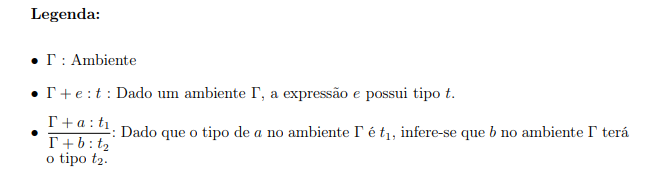
\includegraphics[scale=1]{imagens/ambientesemantico.png}
\end{figure}

\begin{figure}[!ht]
\centering
\caption{Regras de verificação de tipos da linguagem Java.
      \label{fig:4}}
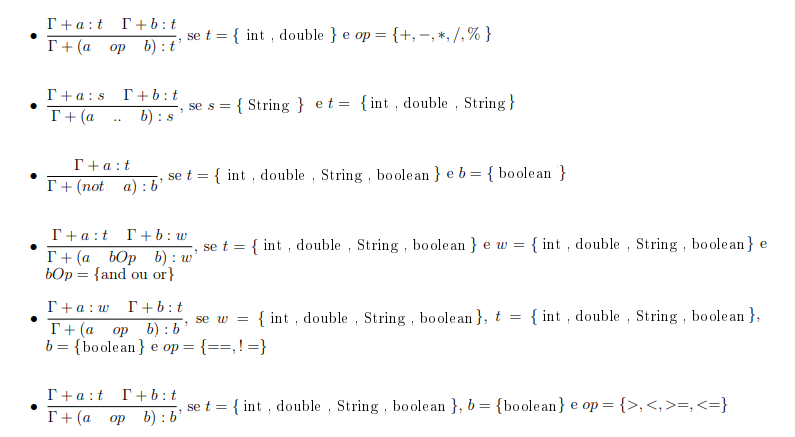
\includegraphics[scale=1]{imagens/ambientesemanticoregras.png}
\end{figure}

\section{Implementação}

A seguir foi feita algumas alterações nos arquivos lexer.mll e parser.mly assim como no ast.ml para realizar a análise de tipos posteriormente.
\subsection{parser.mly}
\begin{terminal}

%{
open Lexing
open Ast
open Sast
%}

%token <int * Lexing.position> LITINT
%token <Lexing.position> INT
%token <float * Lexing.position> LITDOUBLE
%token <Lexing.position> DOUBLE
%token <string * Lexing.position> ID
%token <string * Lexing.position> LITSTRING
%token <Lexing.position> STRING
%token <bool * Lexing.position> LITBOOLEAN
%token <Lexing.position> BOOLEAN
%token <Lexing.position> CLASS
%token <Lexing.position> STATIC
%token <Lexing.position> MAIN NOT
%token <Lexing.position> PUBLIC
%token <Lexing.position> VIRGULA  PONTOEVIRGULA
%token <Lexing.position> APAR FPAR
%token <Lexing.position> IF  ELSE
%token <Lexing.position> WHILE 
%token <Lexing.position> ESCREVA
%token <Lexing.position> LEIA
%token <Lexing.position> FCHAVE
%token <Lexing.position> ACHAVE
%token <Lexing.position> ATRIB
%token <Lexing.position> SOMA
%token <Lexing.position> SUB
%token <Lexing.position> MULT
%token <Lexing.position> DIVISAO
%token <Lexing.position> MENOR
%token <Lexing.position> MENORIGUAL
%token <Lexing.position> IGUAL
%token <Lexing.position> DIFERENTE
%token <Lexing.position> MAIOR
%token <Lexing.position> MAIORIGUAL
%token <Lexing.position> E
%token <Lexing.position> OU
%token <Lexing.position> RETURN
%token <Lexing.position> ACOL FCOL VOID

%token EOF

%left OU
%left E
%left IGUAL DIFERENTE
%left MAIOR MENOR MAIORIGUAL MENORIGUAL
%left SOMA SUB
%left MULT DIVISAO


%start <Sast.expressao Ast.prog> prog

%%

prog: 
	   CLASS ID ACHAVE
            ds = var_decl*
            fs = declaracao_metodo*
            cs = comando_block
          FCHAVE
          EOF { Class (List.flatten ds, fs, cs) }


var_decl :t=tipo ids = separated_nonempty_list(VIRGULA, ID) PONTOEVIRGULA{
                   List.map (fun id -> Var (id,t)) ids
          };

          comando_block :|PUBLIC STATIC VOID  MAIN APAR STRING ACOL FCOL ID FPAR ACHAVE comandos=comando* FCHAVE {comandos};


declaracao_metodo:   STATIC tret = tipo  nome = ID APAR formais = separated_list(VIRGULA, parametro) FPAR 
		   ACHAVE
  			ds = var_decl*
  			cs = comando*
  		FCHAVE {
    			DecFun {
      				fn_nome = nome;
      				fn_tiporet = tret ;
      				fn_formais = formais;
      				fn_locais = List.flatten ds;
      				fn_corpo = cs
    			}
 		}

parametro: t = tipo nome = ID  { (nome, t) }


tipo: t=tipo_simples  { t }

tipo_simples: INT       { TipoInteiro   }
	    | DOUBLE      { TipoDouble }
            | STRING { TipoString }
            | BOOLEAN    { TipoBoolean }

comando: c=comando_atribuicao { c }
       | c=comando_se         { c }
       | c=comando_leia       { c }
       | c=comando_escreva    { c }
       | c=comando_enquanto   { c }
       | c=comando_chamada    { c }
       | c=comando_retorno    { c }


comando_atribuicao: v=expressao ATRIB e=expressao PONTOEVIRGULA {
      CmdAtrib (v,e)
}

comando_se: IF APAR teste=expressao FPAR ACHAVE
               entao=comando*  FCHAVE
               senao=comando_senao?
            { CmdSe (teste, entao, senao) };

comando_senao:
|ELSE ACHAVE comandos=comando* FCHAVE {comandos}

comando_leia: xs=separated_nonempty_list(VIRGULA, expressao)  LEIA APAR   FPAR PONTOEVIRGULA {
                   CmdLeia xs
               }

comando_escreva: ESCREVA APAR xs=separated_nonempty_list(VIRGULA, expressao) FPAR PONTOEVIRGULA {
                 CmdEscreva xs
             }

comando_enquanto: WHILE APAR teste=expressao FPAR ACHAVE
			comandos=comando*
		  FCHAVE { CmdEnquanto (teste,comandos) }


comando_chamada: exp=chamada PONTOEVIRGULA { CmdChamada exp }

comando_retorno: RETURN e=expressao? PONTOEVIRGULA { CmdRetorno e}


expressao:
         | v=variavel     { ExpVar v    }
         | i=LITINT       { ExpInt i    }
	 | f=LITDOUBLE      { ExpDouble f   }
         | s=LITSTRING { ExpString s }
         | b=LITBOOLEAN    { ExpBoolean b }
         | NOT e=LITBOOLEAN {ExpNot e}
	 | e1=expressao op=op e2=expressao { ExpOp (op, e1, e2) }
         | c=chamada      { c }
 	 | APAR e=expressao FPAR { e }

chamada : nome=ID APAR args=separated_list(VIRGULA, expressao) FPAR {
             ExpChamada  (nome, args)}

%inline op:
	| pos = SOMA       { (Soma, pos)       }
        | pos = SUB      { (Sub, pos)      }
        | pos = MULT       { (Mult, pos)       }
        | pos = DIVISAO        { (Divisao, pos)        }
        | pos = MENOR      { (Menor, pos)      }
	| pos = MENORIGUAL { (MenorIgual, pos) }
        | pos = IGUAL      { (Igual, pos)      }
        | pos = DIFERENTE      { (Difer, pos)      }
        | pos = MAIOR      { (Maior, pos)      }
	| pos = MAIORIGUAL { (MaiorIgual, pos) }
        | pos = E          { (AND, pos)        }
        | pos = OU         { (Ou, pos)         }


variavel: x=ID       { VarSimples x }

\end{terminal}
Agora o analisador léxico tem o papel fundamental de passar para as etapas seguintes as posições dos tokens e operadores.  
\subsection{lexer.mll}
\begin{terminal}
{
  open Lexing
  open Printf
  open Parser

  exception Erro of string

  let incr_num_linha lexbuf = 
    let pos = lexbuf.lex_curr_p in
    lexbuf.lex_curr_p <-
      { pos with pos_lnum = pos.pos_lnum + 1;
                 pos_bol = pos.pos_cnum
      }

    let pos_atual lexbuf = lexbuf.lex_start_p

}

let digito = ['0' - '9']
let inteiro = digito+
let double = digito+'.'digito+
let boolean = ("true"|"false")

let letra = ['a' - 'z' 'A' - 'Z']
let identificador = letra ( letra | digito | '_')*

let brancos = [' ' '\t']+
let novalinha = '\r' | '\n' | "\r\n"

let comentario = "--" [^ '\r' '\n' ]*

rule token = parse
  brancos    { token lexbuf }
| novalinha  { incr_num_linha lexbuf; token lexbuf }
| comentario { token lexbuf }
| "/*"       { comentario_bloco 0 lexbuf }
| '('        { APAR (pos_atual lexbuf) }
| '{'        { ACHAVE (pos_atual lexbuf) }
| '}'        { FCHAVE (pos_atual lexbuf) }
| ','	     { VIRGULA (pos_atual lexbuf) }
| ';'        { PONTOEVIRGULA (pos_atual lexbuf) }
| "="	     { ATRIB (pos_atual lexbuf) }
| '+'        { SOMA (pos_atual lexbuf) }
| '-'	     { SUB (pos_atual lexbuf) }
| '*'	     { MULT (pos_atual lexbuf) }
| '['	     { ACOL (pos_atual lexbuf) }
| ']'	     { FCOL (pos_atual lexbuf) }
| '/'	     { DIVISAO (pos_atual lexbuf) }
| ')'        { FPAR (pos_atual lexbuf) }
| '!'        { NOT (pos_atual lexbuf) }
| '>'	     { MAIOR (pos_atual lexbuf) }
| '<'	     { MENOR (pos_atual lexbuf) }
| "=="     { IGUAL (pos_atual lexbuf) }
| "static"  { STATIC (pos_atual lexbuf) }
| "main"  { MAIN (pos_atual lexbuf) }
| ">="	     { MAIORIGUAL (pos_atual lexbuf) }
| "<="	     { MENORIGUAL (pos_atual lexbuf) }
| "!="	     { DIFERENTE (pos_atual lexbuf) }
|"void" { VOID (pos_atual lexbuf) }
| "int"  { INT (pos_atual lexbuf) }
| inteiro as num { let numero = int_of_string num in 
                    LITINT (numero, pos_atual lexbuf)  } 
| "double"     { DOUBLE (pos_atual lexbuf) }
| double as num { let numero = float_of_string num in
		  LITDOUBLE (numero, pos_atual lexbuf) }
| "String" { STRING (pos_atual lexbuf) }
| "boolean"   { BOOLEAN (pos_atual lexbuf) }
| boolean as l { let booleano = bool_of_string l in
		  LITBOOLEAN (booleano, pos_atual lexbuf) }
| "class" { CLASS (pos_atual lexbuf) }
| "public"	     { PUBLIC (pos_atual lexbuf) }
| "System.out.println" { ESCREVA (pos_atual lexbuf) }
| "= s.next"     { LEIA (pos_atual lexbuf) }
| "if"       { IF (pos_atual lexbuf) }
| "&&"	     { E (pos_atual lexbuf) }
| "||"	     { OU (pos_atual lexbuf) }
| "else"    { ELSE (pos_atual lexbuf) }
| "while"    { WHILE (pos_atual lexbuf) }
| "return"   { RETURN (pos_atual lexbuf) }
| identificador as id { ID (id, pos_atual lexbuf) }
| '"'   { let buffer = Buffer.create 1 in
            let str = leia_string buffer lexbuf in
               LITSTRING (str, pos_atual lexbuf) }
| _ { raise (Erro ("Caracter desconhecido: " ^ Lexing.lexeme lexbuf)) }
| eof        { EOF }

and comentario_bloco n = parse
   "*/"      { if n=0 then token lexbuf 
               else comentario_bloco (n-1) lexbuf }
| "/*"       { comentario_bloco (n+1) lexbuf }
| novalinha  { incr_num_linha lexbuf; comentario_bloco n lexbuf }
| _          { comentario_bloco n lexbuf }
| eof        { raise (Erro "Comentário não terminado") }

and leia_string buffer = parse
   '"'      { Buffer.contents buffer}
| "\\t"     { Buffer.add_char buffer '\t'; leia_string buffer lexbuf }
| "\\n"     { Buffer.add_char buffer '\n'; leia_string buffer lexbuf }
| '\\' '"'  { Buffer.add_char buffer '"'; leia_string buffer lexbuf }
| '\\' '\\' { Buffer.add_char buffer '\\'; leia_string buffer lexbuf }
| _ as c    { Buffer.add_char buffer c; leia_string buffer lexbuf }
| eof       { raise (Erro "A string não foi terminada") }

\end{terminal}
\subsection{sast.ml}
\begin{terminal}
open Ast

type expressao =
  | ExpVar of (expressao variavel)
  | ExpInt of int pos
  | ExpDouble of float pos
  | ExpString of string pos
  | ExpBoolean of bool pos
  | ExpNot of bool pos
  | ExpOp of op pos * expressao * expressao
  | ExpChamada of identificador pos * (expressao expressoes)

\end{terminal}
\section{Arquivos Semântico}
Temos a seguir a criação de um módulo capaz de criar e verificar escopos que as linguagens possum afim de criar ambientes para simular os escopos.A cada nova função ou novo comando cria-se um escopo,que pode até ter variáveis com um mesmo identificador,no entanto em contextos diferentes. 
\subsection{tast.ml}
\begin{terminal}
open Ast

type expressao = ExpVar of (expressao variavel) * tipo
              | ExpInt of int * tipo
	      | ExpDouble of float * tipo
              | ExpString of string * tipo
  	      | ExpVoid
              | ExpBoolean of bool * tipo
              | ExpNot of  bool * tipo
              | ExpOp of (op * tipo) * (expressao * tipo) * (expressao * tipo)
              | ExpChamada of identificador * (expressao expressoes) * tipo
\end{terminal}

\subsection{ambiente.ml}
\begin{terminal}
module Tab = Tabsimb
module A = Ast

type entrada_fn = { tipo_fn:  A.tipo;
                    formais: (string * A.tipo) list;
}

type entrada =  EntFun of entrada_fn
             |  EntVar of A.tipo

type t = {
  ambv : entrada Tab.tabela
}

let novo_amb xs = { ambv = Tab.cria xs }

let novo_escopo amb = { ambv = Tab.novo_escopo amb.ambv }

let busca amb ch = Tab.busca amb.ambv ch

let insere_local amb ch t =
  Tab.insere amb.ambv ch (EntVar t)

let insere_param amb ch t =
  Tab.insere amb.ambv ch (EntVar t)

let insere_fun amb nome params resultado =
  let ef = EntFun { tipo_fn = resultado;
                    formais = params }
  in Tab.insere amb.ambv nome ef

\end{terminal}

\subsection{tabsimb.ml}
Também é criado o módulo de tabela de símbolos com o objetivo de inserir, substituir e atualizar símbolos com seus respectivos tipos nos escopos.
\begin{terminal}

type 'a tabela = {
    tbl: (string, 'a) Hashtbl.t;
    pai: 'a tabela option;
}

exception Entrada_existente of string;;

let insere amb ch v =
  if Hashtbl.mem amb.tbl ch
  then raise (Entrada_existente ch)
  else Hashtbl.add amb.tbl ch v

let substitui amb ch v = Hashtbl.replace amb.tbl ch v

let rec atualiza amb ch v =
    if Hashtbl.mem amb.tbl ch
    then Hashtbl.replace amb.tbl ch v
    else match amb.pai with
       None -> failwith "tabsim atualiza: chave nao encontrada"
     | Some a -> atualiza a ch v

let rec busca amb ch =
  try Hashtbl.find amb.tbl ch
  with Not_found ->
    (match amb.pai with
       None -> raise Not_found
     | Some a -> busca a ch)

let rec cria cvs =
  let amb = {
    tbl = Hashtbl.create 5;
    pai = None
  } in
  let _ = List.iter (fun (c,v) -> insere amb c v) cvs
  in amb

let novo_escopo amb_pai = {
  tbl = Hashtbl.create 5;
  pai = Some amb_pai
}
\end{terminal}

\subsection{mainAst.ml}
\begin{terminal}
let parse s =
  let lexbuf = Lexing.from_string s in
  let ast = Parser.prog Lexer.token lexbuf in
  ast

let parse_arq arq =
  let ic = open_in arq in
  let lexbuf = Lexing.from_channel ic in
  let ast = Parser.prog Lexer.token lexbuf in
  let _ = close_in ic in
  ast
\end{terminal}

\subsection{semantico.ml}
\begin{terminal}
module Amb = Ambiente
module A = Ast
module S = Sast
module T = Tast

let rec posicao exp = let open S in
  match exp with
  | ExpVar v -> (match v with
      | A.VarSimples (_,pos) -> pos
    )
  | ExpInt (_,pos) -> pos
  | ExpDouble (_,pos) -> pos
  | ExpString  (_,pos) -> pos
  | ExpBoolean (_,pos) -> pos
  | ExpNot (_,pos) -> pos
  | ExpOp ((_,pos),_,_)  -> pos
  | ExpChamada ((_,pos), _) -> pos

type classe_op = Aritmetico | Relacional | Boolean

let classifica op =
  let open A in
  match op with
    Ou
  | AND -> Boolean
  | Menor
  | MenorIgual
  | Maior
  | MaiorIgual
  | Igual
  | Difer -> Relacional
  | Soma
  | Sub
  | Mult
  | Divisao -> Aritmetico

let msg_erro_pos pos msg =
  let open Lexing in
  let lin = pos.pos_lnum
  and col = pos.pos_cnum - pos.pos_bol - 1 in
  Printf.sprintf "Semantico -> linha %d, coluna %d: %s" lin col msg

let msg_erro nome msg =
  let pos = snd nome in
  msg_erro_pos pos msg

let nome_tipo t =
  let open A in
    match t with
      TipoInteiro -> "inteiro"
    | TipoString -> "string"
    | TipoDouble -> "double"
    | TipoBoolean -> "boolean"
    | TipoVoid -> "void"

let mesmo_tipo pos msg tinf tdec =
  if tinf <> tdec
  then
    let msg = Printf.sprintf msg (nome_tipo tinf) (nome_tipo tdec) in
    failwith (msg_erro_pos pos msg)

let rec infere_exp amb exp =
  match exp with
    S.ExpInt n    -> (T.ExpInt (fst n, A.TipoInteiro), A.TipoInteiro)
  | S.ExpDouble r -> (T.ExpDouble (fst r, A.TipoDouble), A.TipoDouble)
  | S.ExpString s -> (T.ExpString (fst s, A.TipoString), A.TipoString)
  | S.ExpBoolean b   -> (T.ExpBoolean (fst b, A.TipoBoolean), A.TipoBoolean)
  | S.ExpNot nt   -> (T.ExpNot (fst nt, A.TipoBoolean), A.TipoBoolean)
  | S.ExpVar v ->
    (match v with
       A.VarSimples nome ->
       (* Tenta encontrar a definição da variável no escopo local, se não      *)
       (* encontar tenta novamente no escopo que engloba o atual. Prossegue-se *)
       (* assim até encontrar a definição em algum escopo englobante ou até    *)
       (* encontrar o escopo global. Se em algum lugar for encontrado,         *)
       (* devolve-se a definição. Em caso contrário, devolve uma exceção       *)
       let id = fst nome in
         (try (match (Amb.busca amb id) with
               | Amb.EntVar tipo -> (T.ExpVar (A.VarSimples nome, tipo), tipo)
               | Amb.EntFun _ ->
                 let msg = "nome de funcao usado como nome de variavel: " ^ id in
                  failwith (msg_erro nome msg)
             )
          with Not_found ->
                 let msg = "A variavel " ^ id ^ " nao foi declarada" in
                 failwith (msg_erro nome msg)
         )

    )
  | S.ExpOp (op, esq, dir) ->
    let (esq, tesq) = infere_exp amb esq
    and (dir, tdir) = infere_exp amb dir in

    let verifica_aritmetico () =
      (match tesq with
         A.TipoInteiro ->
         let _ = mesmo_tipo (snd op)
                      "O operando esquerdo eh do tipo %s mas o direito eh do tipo %s"
                      tesq tdir
         in tesq (* O tipo da expressão aritmética como um todo *)

       | A.TipoDouble ->
         let _ = mesmo_tipo (snd op)
                      "O operando esquerdo eh do tipo %s mas o direito eh do tipo %s"
                      tesq tdir
         in tesq (* O tipo da expressão aritmética como um todo *)

       | t -> let msg = "um operador aritmetico nao pode ser usado com o tipo " ^
                        (nome_tipo t)
         in failwith (msg_erro_pos (snd op) msg)
      )

    and verifica_relacional () =
      (match tesq with
         A.TipoInteiro
       | A.TipoDouble
       | A.TipoString ->
         let _ = mesmo_tipo (snd op)
                   "O operando esquerdo eh do tipo %s mas o direito eh do tipo %s"
                   tesq tdir
         in A.TipoBoolean (* O tipo da expressão relacional é sempre booleano *)

       | t -> let msg = "um operador relacional nao pode ser usado com o tipo " ^
                        (nome_tipo t)
         in failwith (msg_erro_pos (snd op) msg)
      )

    and verifica_boolean () =
      (match tesq with
         A.TipoBoolean ->
         let _ = mesmo_tipo (snd op)
                   "O operando esquerdo eh do tipo %s mas o direito eh do tipo %s"
                   tesq tdir
         in A.TipoBoolean (* O tipo da expressão lógica é sempre booleano *)

       | t -> let msg = "um operador boolean nao pode ser usado com o tipo " ^
                        (nome_tipo t)
              in failwith (msg_erro_pos (snd op) msg)
      )
    
    in
    let op = fst op in
    let tinf = (match (classifica op) with
          Aritmetico -> verifica_aritmetico ()
        | Relacional -> verifica_relacional ()
        | Boolean -> verifica_boolean ()
      )
    in
      (T.ExpOp ((op,tinf), (esq, tesq), (dir, tdir)), tinf)

    | S.ExpChamada (nome, args) ->
     let rec verifica_parametros ags ps fs =
        match (ags, ps, fs) with
         (a::ags), (p::ps), (f::fs) ->
            let _ = mesmo_tipo (posicao a)
                     "O parametro eh do tipo %s mas deveria ser do tipo %s" p f
            in verifica_parametros ags ps fs
       | [], [], [] -> ()
       | _ -> failwith (msg_erro nome "Numero incorreto de parametros")
     in
     let id = fst nome in
     try
       begin
         let open Amb in

         match (Amb.busca amb id) with
         (* verifica se 'nome' está associada a uma função *)
           Amb.EntFun {tipo_fn; formais} ->
           (* Infere o tipo de cada um dos argumentos *)
           let argst = List.map (infere_exp amb) args
           (* Obtem o tipo de cada parâmetro formal *)
           and tipos_formais = List.map snd formais in
           (* Verifica se o tipo de cada argumento confere com o tipo declarado *)
           (* do parâmetro formal correspondente.                               *)
           let _ = verifica_parametros args (List.map snd argst) tipos_formais
            in (T.ExpChamada (id, (List.map fst argst), tipo_fn), tipo_fn)
         | Amb.EntVar _ -> (* Se estiver associada a uma variável, falhe *)
           let msg = id ^ " eh uma variavel e nao uma funcao" in
           failwith (msg_erro nome msg)
       end
     with Not_found ->
       let msg = "Nao existe a funcao de nome " ^ id in
       failwith (msg_erro nome msg)

let rec verifica_cmd amb tiporet cmd =
  let open A in
  match cmd with
  CmdRetorno exp ->
    (match exp with
     (* Se a função não retornar nada, verifica se ela foi declarada como void *)
       None ->
       let _ = mesmo_tipo (Lexing.dummy_pos)
                   "O tipo retornado eh %s mas foi declarado como %s"
                   TipoVoid tiporet
       in CmdRetorno None
     | Some e ->
       (* Verifica se o tipo inferido para a expressão de retorno confere com o *)
       (* tipo declarado para a função.                                         *)
           let (e1,tinf) = infere_exp amb e in
           let _ = mesmo_tipo (posicao e)
                              "O tipo retornado eh %s mas foi declarado como %s"
                              tinf tiporet
           in CmdRetorno (Some e1)
      )

  | CmdSe (teste, entao, senao) ->
    let (teste1,tinf) = infere_exp amb teste in
    (* O tipo inferido para a expressão 'teste' do condicional deve ser booleano *)
    let _ = mesmo_tipo (posicao teste)
             "O teste do if deveria ser do tipo %s e nao %s"
             TipoBoolean tinf in
    (* Verifica a validade de cada comando do bloco 'então' *)
    let entao1 = List.map (verifica_cmd amb tiporet) entao in
    (* Verifica a validade de cada comando do bloco 'senão', se houver *)
    let senao1 =
        match senao with
          None -> None
        | Some bloco -> Some (List.map (verifica_cmd amb tiporet) bloco)
     in
     CmdSe (teste1, entao1, senao1)

  | CmdAtrib (elem, exp) ->
    (* Infere o tipo da expressão no lado direito da atribuição *)
    let (exp,  tdir) = infere_exp amb exp
    (* Faz o mesmo para o lado esquerdo *)
    and (elem1, tesq) = infere_exp amb elem in
    (* Os dois tipos devem ser iguais *)
    let _ = mesmo_tipo (posicao elem)
                       "Atribuicao com tipos diferentes: %s = %s" tesq tdir
    in CmdAtrib (elem1, exp)

  | CmdChamada exp ->
     let (exp,tinf) = infere_exp amb exp in
     CmdChamada exp

  | CmdLeia exps ->
    (* Verifica o tipo de cada argumento da função 'entrada' *)
    let exps = List.map (infere_exp amb) exps in
    CmdLeia (List.map fst exps)

  | CmdEscreva exps ->
    (* Verifica o tipo de cada argumento da função 'saida' *)
    let exps = List.map (infere_exp amb) exps in
    CmdEscreva (List.map fst exps)

  | CmdEnquanto (teste, corpo) ->
    let (teste1, tinf) = infere_exp amb teste in
    let _ = mesmo_tipo (posicao teste)
	     "O teste do if deveria ser do tipo %s e nao %s"
             TipoBoolean tinf in
    let corpo1 = List.map (verifica_cmd  amb tiporet) corpo in
    CmdEnquanto (teste1, corpo1)

and verifica_fun amb ast =
  let open A in
  match ast with
    A.DecFun {fn_nome; fn_tiporet; fn_formais; fn_locais; fn_corpo} ->
    (* Estende o ambiente global, adicionando um ambiente local *)
    let ambfn = Amb.novo_escopo amb in
    (* Insere os parâmetros no novo ambiente *)
    let insere_parametro (v,t) = Amb.insere_param ambfn (fst v) t in
    let _ = List.iter insere_parametro fn_formais in
    (* Insere as variáveis locais no novo ambiente *)
    let insere_local = function
        (Var (v,t)) -> Amb.insere_local ambfn (fst v)  t in
    let _ = List.iter insere_local fn_locais in
    (* Verifica cada comando presente no corpo da função usando o novo ambiente *)
    let corpo_tipado = List.map (verifica_cmd ambfn fn_tiporet) fn_corpo in
      A.DecFun {fn_nome; fn_tiporet; fn_formais; fn_locais; fn_corpo= corpo_tipado}


let rec verifica_dup xs =
  match xs with
    [] -> []
  | (nome,t)::xs ->
    let id = fst nome in
    if (List.for_all (fun (n,t) -> (fst n) <> id) xs)
    then (id, t) :: verifica_dup xs
    else let msg = "Parametro duplicado " ^ id in
      failwith (msg_erro nome msg)

let insere_declaracao_var amb dec =
  let open A in
    match dec with
        Var (nome, tipo) ->  Amb.insere_local amb (fst nome) tipo

let insere_declaracao_fun amb dec =
  let open A in
    match dec with
      DecFun {fn_nome; fn_tiporet; fn_formais; fn_corpo} ->
        (* Verifica se não há parâmetros duplicados *)
        let formais = verifica_dup fn_formais in
        let nome = fst fn_nome in
        Amb.insere_fun amb nome formais fn_tiporet


(* Lista de cabeçalhos das funções pré definidas *)
let fn_predefs = let open A in [
   ("entrada", [("x", TipoInteiro); ("y", TipoInteiro)], TipoVoid);
   ("saida",   [("x", TipoInteiro); ("y", TipoInteiro)], TipoVoid)
]

(* insere as funções pré definidas no ambiente global *)
let declara_predefinidas amb =
  List.iter (fun (n,ps,tr) -> Amb.insere_fun amb n ps tr) fn_predefs

let semantico ast =
  (* cria ambiente global inicialmente vazio *)
  let amb_global = Amb.novo_amb [] in
  let _ = declara_predefinidas amb_global in
  let (A.Class (decs_globais, decs_funs, corpo)) = ast in
  let _ = List.iter (insere_declaracao_var amb_global) decs_globais in
  let _ = List.iter (insere_declaracao_fun amb_global) decs_funs in
  (* Verificação de tipos nas funções *)
  let decs_funs = List.map (verifica_fun amb_global) decs_funs in
  (* Verificação de tipos na função principal *)
  let corpo = List.map (verifica_cmd amb_global A.TipoVoid) corpo in
     (A.Class (decs_globais, decs_funs, corpo),  amb_global)
\end{terminal}


\subsection{semanticoTest}
A seguir a implementação do arquivo de teste do analisador semântico.No OCaml é chamada a função verifica tipos para visualização da árvore tipada  gerada.
\begin{terminal}open Printf
open Lexing

open Ast
exception Erro_Sintatico of string

module S = MenhirLib.General (* Streams *)
module I = Parser.MenhirInterpreter

open Semantico

let message =
  fun s ->
    match s with
    | 1 ->
        "Erro Sintático - erro após class, nome da classe esperado \n"
    | 2 ->
        "Erro Sintático  - erro após identificador da classe, abre chave esperado \n"
    | 3 ->
        "Erro Sintático - erro após abre chave da classe \n"
    | 10 ->
        "Erro Sintático - erro após declaração de tipo da variavel \n"
    | 11 ->
        "Erro Sintático - ponto e virgula ou virgula esperado \n"
    | 12 ->
        "Erro Sintático - erro após a virgula \n"
    | 8 ->
        "Erro Sintático - erro na declaração de variavel \n"
    | 17 ->
        "Erro Sintático - erro no inicio da classe, espera-se declaracao de metodos após variaveis \n"
    | 18 ->
        "Erro Sintático - erro após static, tipo esperado \n"
    | 19 ->
        "Erro Sintático - erro após identificador, tipo esperado \n"
    | 20 ->
        "Erro Sintático - erro após identificador, abre parenteses esperado \n"
    | 21 ->
        "Erro Sintático - parametros válidos esperados \n"
    | 22 ->
        "Erro Sintático - identificador esperado após o tipo \n"
    | 25 ->
        "Erro Sintático - fecha parenteses ou virgula esperado no parametro \n"
    | 26 ->
        "Erro Sintático - erro nos parametros, após a virgula \n"
    | 29 ->
        "Erro Sintático -erro após fecha parenteses do metodo \n"
    | 32 ->
        "Erro Sintático - erro depois do while e antes do parenteses \n"
    | 33 ->
        "Erro Sintático - erro na expressão do while  \n"
    | 77 ->
        "Erro Sintático - erro na expressão do while  \n"
    | 78 ->
        "Erro Sintático - erro antes abre chave do while  \n"
    | 79 ->
        "Erro Sintático - erro após abre chave do while  \n"
    | 30 ->
        "Erro Sintático - erro após abre chave do método \n"
    | 31 ->
        "Erro Sintático - erro no método entre os comandos e as declarações de variaveis  \n"
    | 80 ->
        "Erro Sintático - expressão esperada no return \n"
    | 116 ->
        "Erro Sintático - erro apos comando \n"
    | 83 ->
        "Erro Sintático - operador aritmético esperado após a expressão   \n"
    | 34 ->
        "Erro Sintático - booleano esperado após o not \n"
    | 105 ->
        "Erro Sintático - operador aritmético esperado após a expressão  \n"
    | 75 ->
        "Erro Sintático - erro na expressão do comando de leitura \n"
    | 74 ->
        "Erro Sintático - operador aritmético esperado após a expressão   \n"
    | 94 ->
        "Erro Sintático - erro no comando de leitura, = esperado \n"
    | 45 ->
        "Erro Sintático - expressao esperada após o operador SUB \n"
    | 46 ->
        "Erro Sintático - operador aritmético esperado após a expressão  \n"
    | 52 ->
        "Erro Sintático - expressao esperada após o operador SOMA \n"
    | 53 ->
        "Erro Sintático - operador aritmético esperado após a expressão\n"
    | 54 ->
        "Erro Sintático - expressao esperada após o operador OU \n"
    | 55 ->
        "Erro Sintático - operador aritmético esperado após a expressão \n"
    | 47 ->
        "Erro Sintático - expressao esperada após o operador MULT \n"
    | 56 ->
        "Erro Sintático - expressao esperada após o operador MENORIGUAL \n"
    | 57 ->
        "Erro Sintático - operador aritmético esperado após a expressão \n"
    | 58 ->
        "Erro Sintático - expressao esperada após o operador MENOR \n"
    | 59 ->
        "Erro Sintático - operador aritmético esperado após a expressão \n"
    | 60 ->
        "Erro Sintático - expressao esperada após o operador MAIORIGUAL \n"
    | 61 ->
        "Erro Sintático - operador aritmético esperado após a expressão \n"
    | 62 ->
        "Erro Sintático - expressao esperada após o operador MAIOR \n"
    | 63 ->
        "Erro Sintático - operador aritmético esperado após a expressão  \n"
    | 95 ->
        "Erro Sintático - erro após comando de leitura s.next, abre parênteses esperado \n"
    | 96 ->
        "Erro Sintático - erro após comando de leitura s.next,fecha parenteses esperado \n"
    | 97 ->
        "Erro Sintático - ponto e virgula esperado\n"
    | 64 ->
        "Erro Sintático - expressao esperada após o operador IGUAL \n"
    | 65 ->
        "Erro Sintático - operador aritmético esperado após a expressão \n"
    | 66 ->
        "Erro Sintático - expressao esperada após o operador E \n"
    | 67 ->
        "Erro Sintático - operador aritmético esperado após a expressão \n"
    | 50 ->
        "Erro Sintático - expressão esperada apos divisão \n"
    | 68 ->
        "Erro Sintático - expressão esperada \n"
    | 69 ->
        "Erro Sintático - operador aritmético esperado após a expressão \n"
    | 106 ->
        "Erro Sintático -erro depois de atribuir expressão \n"
    | 107 ->
        "Erro Sintático - erro na expressão depois de atribuida \n"
    | 84 ->
        "Erro Sintático - abre parênteses esperado após o if \n"
    | 85 ->
        "Erro Sintático - expressão esperada após abre parenteses do if\n"
    | 86 ->
        "Erro Sintático - erro na expressão do if, fecha parenteses esperado \n"
    | 87 ->
        "Erro Sintático - erro após fechar parênteses da expressão do if. Abre chave esperado \n"
    | 88 ->
        "Erro Sintático - erro após abre chave do if \n"
    | 100 ->
        "Erro Sintático - erro após fechar chave do if \n"
    | 101 ->
        "Erro Sintático - erro entre o else e o abre chave\n"
    | 102 ->
        "Erro Sintático - erro após abre chave do else\n"
    | 40 ->
        "Erro Sintático -erro após identificador \n"
    | 41 ->
        "Erro Sintático - erro dentro da expressão entre parênteses \n"
    | 72 ->
        "Erro Sintático - fecha parenteses esperado \n"
    | 118 ->
        "Erro Sintático - erro na chamada de função \n"
    | 143 ->
        "Erro Sintático - erro no método \n"
    | 89 ->
        "Erro Sintático - erro antes abre parenteses do println \n"
    | 90 ->
        "Erro Sintático - erro após abre parenteses do println \n"
    | 91 ->
        "Erro Sintático - fecha parênteses  esperado após o println  \n"
    | 92 ->
        "Erro Sintático - ponto e vírgula esperado após o println \n"
    | 42 ->
        "Erro Sintático - erro na expressão entre parênteses \n"
    | 44 ->
        "Erro Sintático - erro entre a expressão e o operador \n"
    | 127 ->
        "Erro Sintático -static esperado no método main após public \n"
    | 128 ->
        "Erro Sintático -void esperado no método main \n"
    | 129 ->
        "Erro Sintático - main esperado no método main\n"
    | 130 ->
        "Erro Sintático - abre parenteses esperado no método main \n"
    | 131 ->
        "Erro Sintático - palavra String esperada \n"
    | 132 ->
        "Erro Sintático - abre colchete esperado no método main\n"
    | 133 ->
        "Erro Sintático - fecha colchete esperado no método main\n"
    | 134 ->
        "identificador esperado no método main"
    | 135 ->
        "fecha parenteses esperado no método main"
    | 136 ->
        "Erro Sintático - abre chave esperado \n"
    | 137 ->
        "comando esperado"
    | 140 ->
        "Erro no fim do corpo da classe\n"
    | 141 ->
        "Erro depois da classe\n"
    | _ ->
        raise Not_found

let posicao lexbuf =
    let pos = lexbuf.lex_curr_p in
    let lin = pos.pos_lnum
    and col = pos.pos_cnum - pos.pos_bol - 1 in
    sprintf "linha %d, coluna %d" lin col

(* [pilha checkpoint] extrai a pilha do autômato LR(1) contida em checkpoint *)

let pilha checkpoint =
  match checkpoint with
  | I.HandlingError amb -> I.stack amb
  | _ -> assert false (* Isso não pode acontecer *)

let estado checkpoint : int =
  match Lazy.force (pilha checkpoint) with
  | S.Nil -> (* O parser está no estado inicial *)
     0
  | S.Cons (I.Element (s, _, _, _), _) ->
     I.number s

let sucesso v = Some v

let falha lexbuf (checkpoint : (Sast.expressao Ast.prog) I.checkpoint) =
  let estado_atual = estado checkpoint in
  let msg = message estado_atual in
  raise (Erro_Sintatico (Printf.sprintf "%d - %s.\n"
                                      (Lexing.lexeme_start lexbuf) msg))

let loop lexbuf resultado =
  let fornecedor = I.lexer_lexbuf_to_supplier Lexer.token lexbuf in
  I.loop_handle sucesso (falha lexbuf) fornecedor resultado


let parse_com_erro lexbuf =
  try
    Some (loop lexbuf (Parser.Incremental.prog lexbuf.lex_curr_p))
  with
  | Lexer.Erro msg ->
     printf "Erro lexico na %s:\n\t%s\n" (posicao lexbuf) msg;
     None
  | Erro_Sintatico msg ->
     printf "Erro sintático na %s %s\n" (posicao lexbuf) msg;
     None

let parse s =
  let lexbuf = Lexing.from_string s in
  let ast = parse_com_erro lexbuf in
  ast

let parse_arq nome =
  let ic = open_in nome in
  let lexbuf = Lexing.from_channel ic in
  let ast = parse_com_erro lexbuf in
  let _ = close_in ic in
  ast

let verifica_tipos nome =
  let ast = parse_arq nome in
  match ast with
    Some (Some ast) -> semantico ast
  | _ -> failwith "Nada a fazer!\n"

\end{terminal}
\subsubsection{Script para compilação}
 Neste trabalho é utilizado o menhirLib, ocamlfind e ocamlbuild para compilar todos os arquivos necessários.
Foi feito um script com os comandos necessários para compilar e testar o analisador semântico.Para executar digite no terminal ./script.sh .
\begin{terminal}
#!/bin/bash
rm -rf  _build  *.byte
 ocamlbuild -use-ocamlfind -use-menhir -menhir "menhir --table" -package menhirLib semanticoTest.byte
rlwrap ocaml
# pra dar permissao pro script rodar digita no terminal chmod 777 exemplo1.sh

\end{terminal}

\chapter{Intérprete}
A funcão do intérprete é similar à do analisador semântico, com a diferença que, ao invés de fazer análise e inferência de tipos, será
feita a avaliação das expressões sem se preocupar com qualquer tipo de erro, pois já que
o código passou por todas as etapas anteriores do compilador ele não possui erros que o
impedem de ser executado. Nele observamos a preocupação em variáveis não inicializadas ou rótulos de variáveis já utilizadas, assim como tipos que o usuário por ventura digite errado.
O passo a passo para construir o intérprete a partir do semântico é descrito a seguir:
 \begin{terminal}
1 - Copiar pasta do semântico para uma nova pasta.
2 - Copiar os arquivos semantico.ml, semantico.mli e semanticoTest.ml para
interprete.ml, interprete.mli e interpreteTest.ml, respectivamente.
3 - Copiar os arquivos ambiente.ml e ambiente.mli para ambInterp.ml e
ambInterp.mli.
Visualize a árvore resultante do semântico para algum arquivo de interesse
.
- Em ambInterp.ml:
- Alterar 'entrada' para envolver valores
- Inserir 'atualiza_var'
Em interprete.ml:
- renomear a fç semantico para interprete
- alterar fn_predefs
- alterar 'declara_predefinidas'
- alterar 'insere_declaracao_var'
- renomear todas as ocorrências de 'verifica_dup' para 'obtem_formais' e
alterar o corpo;
- alterar 'insere_declaracao_fun'
- alterar 'interprete', removendo 'let decs_funs'
- alterar 'tast.ml' para incluir 'ExpVoid'
- renomear todas as ocorrências de 'verifica_cmd' para 'interpreta_cmd'
e altere o corpo
- renomear todas as ocorrências de 'infere_exp' para 'interpreta_exp'
renomear todas as ocorrências
- Inserir 'obtem_nome_var'
- alterar ''
- Remover 'posicao', 'msg_erro_pos', 'msg_erro' e 'nome_tipo'
\end{terminal}

\section{Arquivos do intérprete}
A seguir os arquivos alterados para construção do intérprete.
\subsection{ambInterp.ml}
Antes no analisador semântico guardávamos apenas o tipo e os identificadores, agora guardamos os comandos e valores das funções na tabela.
\begin{terminal}
module Tab = Tabsimb
module A = Ast
module T = Tast

type entrada_fn = {
  tipo_fn:  A.tipo;
  formais: (A.identificador * A.tipo) list;
  locais:  A.declaracoes;
  corpo: T.expressao A.comandos
}

type entrada =  EntFun of entrada_fn
                        |  EntVar of A.tipo * (T.expressao option)

type t = {
  ambv : entrada Tab.tabela
}

let novo_amb xs = { ambv = Tab.cria xs }

let novo_escopo amb = { ambv = Tab.novo_escopo amb.ambv }

let busca amb ch = Tab.busca amb.ambv ch

let atualiza_var amb ch t v =
  Tab.atualiza amb.ambv ch (EntVar (t,v))

let insere_local amb nome t v =
  Tab.insere amb.ambv nome (EntVar (t,v))

let insere_param amb nome t v =
  Tab.insere amb.ambv nome (EntVar (t,v))

let insere_fun amb nome params locais resultado corpo =
  let ef = EntFun { tipo_fn = resultado;
                    formais = params;
                    locais = locais;
                    corpo = corpo }
  in Tab.insere amb.ambv nome ef

\end{terminal}
\subsection{interprete.ml}
\begin{terminal}
module Amb = AmbInterp
module A = Ast
module S = Sast
module T = Tast

exception Valor_de_retorno of T.expressao

let obtem_nome_tipo_var exp = let open T in
  match exp with
  | ExpVar (v,tipo) ->
    (match v with
      | A.VarSimples (nome,_) -> (nome,tipo)
    )
  | _ -> failwith "obtem_nome_tipo_var: nao eh variavel"

let pega_int exp =
  match exp with
  |  T.ExpInt (i,_) -> i
  | _ -> failwith "pega_int: nao eh inteiro"

let pega_float exp =
  match exp with
  |  T.ExpDouble (i,_) -> i
  | _ -> failwith "pega_float: nao eh double"

let pega_string exp =
  match exp with
  |  T.ExpString (s,_) -> s
  | _ -> failwith "pega_string: nao eh string"

let pega_bool exp =
  match exp with
  |  T.ExpBoolean (b,_) -> b
  |  T.ExpNot (nt,_) -> nt
  | _ -> failwith "pega_bool: nao eh booleano"

type classe_op = Aritmetico | Relacional | Boolean

let classifica op =
  let open A in
  match op with
    Ou
  | AND -> Boolean
  | Menor
  | MenorIgual
  | Maior
  | MaiorIgual
  | Igual
  | Difer -> Relacional
  | Soma
  | Sub
  | Mult
  | Divisao -> Aritmetico


let rec interpreta_exp amb exp =
  let open A in
  let open T in
  match exp with
  | ExpVoid
  | ExpInt _
  | ExpDouble _
  | ExpString _
  | ExpNot _   -> exp
  | ExpBoolean _   -> exp
  | ExpVar _ ->
       let (id,tipo) = obtem_nome_tipo_var exp in
    (* Tenta encontrar o valor da variável no escopo local, se não      *)
    (* encontrar, tenta novamente no escopo que engloba o atual. Prossegue-se *)
    (* assim até encontrar o valor em algum escopo englobante ou até    *)
    (* encontrar o escopo global. Se em algum lugar for encontrado,         *)
    (* devolve-se o valor. Em caso contrário, devolve uma exceção       *)
    (match (Amb.busca amb id) with
     | Amb.EntVar (tipo, v) ->
       (match v with
        | None -> failwith ("variável nao inicializada: " ^ id)
        | Some valor -> valor
       )
     |  _ -> failwith "interpreta_exp: expvar"
    )
  | ExpOp ((op,top), (esq, tesq), (dir,tdir)) ->
    let  vesq = interpreta_exp amb esq
    and vdir = interpreta_exp amb dir in

    let interpreta_aritmetico () =
      (match tesq with
	| TipoInteiro ->
         (match op with
          | Soma ->     ExpInt (pega_int vesq + pega_int vdir, top)
          | Sub -> ExpInt (pega_int vesq - pega_int vdir, top)
          | Mult ->     ExpInt (pega_int vesq * pega_int vdir, top)
          | Divisao  ->      ExpInt (pega_int vesq / pega_int vdir, top)
          | _ -> failwith "interpreta_aritmetico"
         )

       | TipoDouble ->
         (match op with
          | Soma ->     ExpInt (pega_int vesq + pega_int vdir, top)
          | Sub -> ExpInt (pega_int vesq - pega_int vdir, top)
          | Mult ->     ExpInt (pega_int vesq * pega_int vdir, top)
          | Divisao  ->      ExpInt (pega_int vesq / pega_int vdir, top)
          | _ -> failwith "interpreta_aritmetico"
         )
        | _ -> failwith "interpreta_aritmetico"
      )

    and interpreta_relacional () =
      (match tesq with
       | TipoInteiro ->
         (match op with
          | Menor -> ExpBoolean (pega_int vesq < pega_int vdir, top)
	  | MenorIgual -> ExpBoolean (pega_int vesq <= pega_int vdir, top)
          | Maior  -> ExpBoolean (pega_int vesq > pega_int vdir, top)
          | MaiorIgual  -> ExpBoolean (pega_int vesq >= pega_int vdir, top)
          | Igual   -> ExpBoolean (pega_int vesq == pega_int vdir, top)
          | Difer   -> ExpBoolean (pega_int vesq != pega_int vdir, top)
          | _ -> failwith "interpreta_relacional"
         )

       | TipoDouble ->
         (match op with
          | Menor -> ExpBoolean (pega_float vesq < pega_float vdir, top)
	  | MenorIgual -> ExpBoolean (pega_float vesq <= pega_float vdir, top)
          | Maior  -> ExpBoolean (pega_float vesq > pega_float vdir, top)
          | MaiorIgual  -> ExpBoolean (pega_float vesq >= pega_float vdir, top)
          | Igual   -> ExpBoolean (pega_float vesq == pega_float vdir, top)
          | Difer   -> ExpBoolean (pega_float vesq != pega_float vdir, top)

          | _ -> failwith "interpreta_relacional"
         )

       | TipoString ->
         (match op with
          | Menor -> ExpBoolean (pega_string vesq < pega_string vdir, top)
          | MenorIgual -> ExpBoolean (pega_string vesq <= pega_string vdir, top)
          | Maior  -> ExpBoolean (pega_string vesq > pega_string vdir, top)
          | MaiorIgual  -> ExpBoolean (pega_string vesq >= pega_string vdir, top)
          | Igual   -> ExpBoolean (pega_string vesq == pega_string vdir, top)
          | Difer   -> ExpBoolean (pega_string vesq != pega_string vdir, top)

          | _ -> failwith "interpreta_relacional"
         )
       | TipoBoolean ->
         (match op with
          | Menor -> ExpBoolean (pega_bool vesq < pega_bool vdir, top)
          | MenorIgual -> ExpBoolean (pega_bool vesq <= pega_bool vdir, top)
          | Maior  -> ExpBoolean (pega_bool vesq > pega_bool vdir, top)
          | MaiorIgual  -> ExpBoolean (pega_bool vesq >= pega_bool vdir, top)
          | Igual   -> ExpBoolean (pega_bool vesq == pega_bool vdir, top)
          | Difer   -> ExpBoolean (pega_bool vesq != pega_bool vdir, top)


          | _ -> failwith "interpreta_relacional"
         )
       | _ ->  failwith "interpreta_relacional"
      )

    and interpreta_boolean () =
      (match tesq with
       | TipoBoolean ->
         (match op with
          | Ou -> ExpBoolean (pega_bool vesq || pega_bool vdir, top)
          | AND ->   ExpBoolean (pega_bool vesq && pega_bool vdir, top)
          | _ ->  failwith "interpreta_boolean"
         )
       | _ ->  failwith "interpreta_boolean"
      )
    
    in
    let valor = (match (classifica op) with
          Aritmetico -> interpreta_aritmetico ()
        | Relacional -> interpreta_relacional ()
        | Boolean -> interpreta_boolean ()
      )
    in
      valor

  | ExpChamada (id, args, tipo) ->
    let open Amb in
    ( match (Amb.busca amb id) with
      | Amb.EntFun {tipo_fn; formais; locais; corpo} ->
           (* Interpreta cada um dos argumentos *)
           let vargs = List.map (interpreta_exp amb) args in
           (* Associa os argumentos aos parâmetros formais *)
           let vformais = List.map2 (fun (n,t) v -> (n, t, Some v)) formais vargs
           in interpreta_fun amb id vformais locais corpo
      | _ -> failwith "interpreta_exp: expchamada"
    )

and interpreta_fun amb fn_nome fn_formais fn_locais fn_corpo =
  let open A in
 (* Estende o ambiente global, adicionando um ambiente local *)
  let ambfn = Amb.novo_escopo amb in
   let insere_local  d =
    match d with
      (Var (v,t)) -> Amb.insere_local ambfn (fst v)  t None
  in
  (* Associa os argumentos aos parâmetros e insere no novo ambiente *)
  let insere_parametro (n,t,v) = Amb.insere_param ambfn n t v in
  let _ = List.iter insere_parametro fn_formais in
  (* Insere as variáveis locais no novo ambiente *)
    let _ = List.iter insere_local fn_locais in
    (* Interpreta cada comando presente no corpo da função usando o novo
       ambiente *)
  try
    let _ = List.iter (interpreta_cmd ambfn) fn_corpo in T.ExpVoid
    with
       Valor_de_retorno expret -> expret

and interpreta_cmd amb cmd =
  let open A in
  let open T in
  match cmd with
    CmdRetorno exp ->
    (* Levantar uma exceção foi necessária pois, pela semântica do comando de
        retorno, sempre que ele for encontrado em uma função, a computação
        deve parar retornando o valor indicado, sem realizar os demais comandos.
    *)
    (match exp with
     (* Se a função não retornar nada, então retorne ExpVoid *)
       None -> raise (Valor_de_retorno ExpVoid)
     | Some e ->
       (* Avalia a expressão e retorne o resultado *)
       let e1 = interpreta_exp amb e in
       raise (Valor_de_retorno e1)
    )

  | CmdSe (teste, entao, senao) ->
    let teste1 = interpreta_exp amb teste in
    (match teste1 with
       ExpBoolean (true,_) ->
       (* Interpreta cada comando do bloco 'então' *)
       List.iter (interpreta_cmd amb) entao
     | _ ->
       (* Interpreta cada comando do bloco 'senão', se houver *)
       (match senao with
          None -> ()
        | Some bloco -> List.iter (interpreta_cmd amb) bloco
       )
    )

  | CmdAtrib (elem, exp) ->
    (* Interpreta o lado direito da atribuição *)
    let exp = interpreta_exp amb exp
    (* Faz o mesmo para o lado esquerdo *)
    and (elem1,tipo) = obtem_nome_tipo_var elem in
    Amb.atualiza_var amb elem1 tipo (Some exp)

  | CmdChamada exp -> ignore( interpreta_exp amb exp)

  | CmdLeia exps ->
    (* Obtem os nomes e os tipos de cada um dos argumentos *)
    let nts = List.map (obtem_nome_tipo_var) exps in
    let leia_var (nome,tipo) =
      let valor =
        (match tipo with
         | A.TipoInteiro    -> T.ExpInt    (read_int (),  tipo)
	 | A.TipoDouble    -> T.ExpDouble    (read_float (),  tipo)
         | A.TipoString -> T.ExpString (read_line (), tipo)
         | _ -> failwith "leia_var: nao implementado"
        )
      in  Amb.atualiza_var amb nome tipo (Some valor)
    in
    (* Lê o valor para cada argumento e atualiza o ambiente *)
    List.iter leia_var nts


  | CmdEscreva exps ->
    (* Interpreta cada argumento da função 'saida' *)
    let exps = List.map (interpreta_exp amb) exps in
    let imprima exp =
      (match exp with
       | T.ExpInt (n,_) ->      let _ = print_int n in print_string " "
       | T.ExpDouble (r,_) ->      let _ = print_float r in print_string " "
       | T.ExpString (s,_) -> let _ = print_string s in print_string " "
       | T.ExpBoolean (b,_) ->
         let _ = print_string (if b then "true" else "false")
         in print_string " "
        | T.ExpNot (not,_) ->
         let _ = print_string (if not then "false" else "true")
         in print_string " "
          | _ -> failwith "imprima: nao implementado"
      )
    in
    let _ = List.iter imprima exps in
    print_newline ()

    | CmdEnquanto (cond, cmds) ->
        let rec laco cond cmds =
          let condResp = interpreta_exp amb cond in
                (match condResp with
                  | ExpBoolean (true,_) ->
                      (* Interpreta cada comando do bloco 'então' *)
                      let _ = List.iter (interpreta_cmd amb) cmds in
                        laco cond cmds
          | ExpNot (false,_) ->
                      (* Interpreta cada comando do bloco 'então' *)
                      let _ = List.iter (interpreta_cmd amb) cmds in
                        laco cond cmds
                  | _ -> ())
        in laco cond cmds

let insere_declaracao_var amb dec =
    match dec with
        A.Var (nome, tipo) ->  Amb.insere_local amb (fst nome) tipo None

let insere_declaracao_fun amb dec =
  let open A in
    match dec with
      DecFun {fn_nome; fn_tiporet; fn_formais; fn_locais; fn_corpo} ->
        let nome = fst fn_nome in
        let formais = List.map (fun (n,t) -> ((fst n), t)) fn_formais in
        Amb.insere_fun amb nome formais fn_locais fn_tiporet fn_corpo


(* Lista de cabeçalhos das funções pré definidas *)
let fn_predefs = let open A in [
   ("entrada", [("x", TipoInteiro); ("y", TipoInteiro)], TipoVoid, []);
   ("saida",   [("x", TipoInteiro); ("y", TipoInteiro)], TipoVoid, [])
]

(* insere as funções pré definidas no ambiente global *)
let declara_predefinidas amb =
  List.iter (fun (n,ps,tr,c) -> Amb.insere_fun amb n ps [] tr c) fn_predefs

let interprete ast =
  (* cria ambiente global inicialmente vazio *)
  let amb_global = Amb.novo_amb [] in
  let _ = declara_predefinidas amb_global in
  let (A.Class (decs_globais, decs_funs, corpo)) = ast in
  let _ = List.iter (insere_declaracao_var amb_global) decs_globais in
  let _ = List.iter (insere_declaracao_fun amb_global) decs_funs in
  (* Interpreta a função principal *)
  let resultado = List.iter (interpreta_cmd amb_global) corpo in
  resultado


\end{terminal}
Para testarmos o interpretador foi criado um arquivo que através da função interprete no Ocaml nos possibilita executar o programa.
\subsection{interpreteTeste.ml}
\begin{terminal}
open Printf
open Lexing

open Ast
exception Erro_Sintatico of string

module S = MenhirLib.General (* Streams *)
module I = Parser.MenhirInterpreter

open Semantico

let message =
  fun s ->
    match s with
    | 1 ->
        "Erro Sintático - erro após class, nome da classe esperado \n"
    | 2 ->
        "Erro Sintático  - erro após identificador da classe, abre chave esperado \n"
    | 3 ->
        "Erro Sintático - erro após abre chave da classe \n"
    | 10 ->
        "Erro Sintático - erro após declaração de tipo da variavel \n"
    | 11 ->
        "Erro Sintático - ponto e virgula ou virgula esperado \n"
    | 12 ->
        "Erro Sintático - erro após a virgula \n"
    | 8 ->
        "Erro Sintático - erro na declaração de variavel \n"
    | 17 ->
        "Erro Sintático - erro no inicio da classe, espera-se declaracao de metodos após variaveis \n"
    | 18 ->
        "Erro Sintático - erro após static, tipo esperado \n"
    | 19 ->
        "Erro Sintático - erro após identificador, tipo esperado \n"
    | 20 ->
        "Erro Sintático - erro após identificador, abre parenteses esperado \n"
    | 21 ->
        "Erro Sintático - parametros válidos esperados \n"
    | 22 ->
        "Erro Sintático - identificador esperado após o tipo \n"
    | 25 ->
        "Erro Sintático - fecha parenteses ou virgula esperado no parametro \n"
    | 26 ->
        "Erro Sintático - erro nos parametros, após a virgula \n"
    | 29 ->
        "Erro Sintático -erro após fecha parenteses do metodo \n"
    | 32 ->
        "Erro Sintático - erro depois do while e antes do parenteses \n"
    | 33 ->
        "Erro Sintático - erro na expressão do while  \n"
    | 77 ->
        "Erro Sintático - erro na expressão do while  \n"
    | 78 ->
        "Erro Sintático - erro antes abre chave do while  \n"
    | 79 ->
        "Erro Sintático - erro após abre chave do while  \n"
    | 30 ->
        "Erro Sintático - erro após abre chave do método \n"
    | 31 ->
        "Erro Sintático - erro no método entre os comandos e as declarações de variaveis  \n"
    | 80 ->
        "Erro Sintático - expressão esperada no return \n"
    | 116 ->
        "Erro Sintático - erro apos comando \n"
    | 83 ->
        "Erro Sintático - operador aritmético esperado após a expressão   \n"
    | 34 ->
        "Erro Sintático - booleano esperado após o not \n"
    | 105 ->
        "Erro Sintático - operador aritmético esperado após a expressão  \n"
    | 75 ->
        "Erro Sintático - erro na expressão do comando de leitura \n"
    | 74 ->
        "Erro Sintático - operador aritmético esperado após a expressão   \n"
    | 94 ->
        "Erro Sintático - erro no comando de leitura, = esperado \n"
    | 45 ->
        "Erro Sintático - expressao esperada após o operador SUB \n"
    | 46 ->
        "Erro Sintático - operador aritmético esperado após a expressão  \n"
    | 52 ->
        "Erro Sintático - expressao esperada após o operador SOMA \n"
    | 53 ->
        "Erro Sintático - operador aritmético esperado após a expressão\n"
    | 54 ->
        "Erro Sintático - expressao esperada após o operador OU \n"
    | 55 ->
        "Erro Sintático - operador aritmético esperado após a expressão \n"
    | 47 ->
        "Erro Sintático - expressao esperada após o operador MULT \n"
    | 56 ->
        "Erro Sintático - expressao esperada após o operador MENORIGUAL \n"
    | 57 ->
        "Erro Sintático - operador aritmético esperado após a expressão \n"
    | 58 ->
        "Erro Sintático - expressao esperada após o operador MENOR \n"
    | 59 ->
        "Erro Sintático - operador aritmético esperado após a expressão \n"
    | 60 ->
        "Erro Sintático - expressao esperada após o operador MAIORIGUAL \n"
    | 61 ->
        "Erro Sintático - operador aritmético esperado após a expressão \n"
    | 62 ->
        "Erro Sintático - expressao esperada após o operador MAIOR \n"
    | 63 ->
        "Erro Sintático - operador aritmético esperado após a expressão  \n"
    | 95 ->
        "Erro Sintático - erro após comando de leitura s.next, abre parênteses esperado \n"
    | 96 ->
        "Erro Sintático - erro após comando de leitura s.next,fecha parenteses esperado \n"
    | 97 ->
        "Erro Sintático - ponto e virgula esperado\n"
    | 64 ->
        "Erro Sintático - expressao esperada após o operador IGUAL \n"
    | 65 ->
        "Erro Sintático - operador aritmético esperado após a expressão \n"
    | 66 ->
        "Erro Sintático - expressao esperada após o operador E \n"
    | 67 ->
        "Erro Sintático - operador aritmético esperado após a expressão \n"
    | 50 ->
        "Erro Sintático - expressão esperada apos divisão \n"
    | 68 ->
        "Erro Sintático - expressão esperada \n"
    | 69 ->
        "Erro Sintático - operador aritmético esperado após a expressão \n"
    | 106 ->
        "Erro Sintático -erro depois de atribuir expressão \n"
    | 107 ->
        "Erro Sintático - erro na expressão depois de atribuida \n"
    | 84 ->
        "Erro Sintático - abre parênteses esperado após o if \n"
    | 85 ->
        "Erro Sintático - expressão esperada após abre parenteses do if\n"
    | 86 ->
        "Erro Sintático - erro na expressão do if, fecha parenteses esperado \n"
    | 87 ->
        "Erro Sintático - erro após fechar parênteses da expressão do if. Abre chave esperado \n"
    | 88 ->
        "Erro Sintático - erro após abre chave do if \n"
    | 100 ->
        "Erro Sintático - erro após fechar chave do if \n"
    | 101 ->
        "Erro Sintático - erro entre o else e o abre chave\n"
    | 102 ->
        "Erro Sintático - erro após abre chave do else\n"
    | 40 ->
        "Erro Sintático -erro após identificador \n"
    | 41 ->
        "Erro Sintático - erro dentro da expressão entre parênteses \n"
    | 72 ->
        "Erro Sintático - fecha parenteses esperado \n"
    | 118 ->
        "Erro Sintático - erro na chamada de função \n"
    | 143 ->
        "Erro Sintático - erro no método \n"
    | 89 ->
        "Erro Sintático - erro antes abre parenteses do println \n"
    | 90 ->
        "Erro Sintático - erro após abre parenteses do println \n"
    | 91 ->
        "Erro Sintático - fecha parênteses  esperado após o println  \n"
    | 92 ->
        "Erro Sintático - ponto e vírgula esperado após o println \n"
    | 42 ->
        "Erro Sintático - erro na expressão entre parênteses \n"
    | 44 ->
        "Erro Sintático - erro entre a expressão e o operador \n"
    | 127 ->
        "Erro Sintático -static esperado no método main após public \n"
    | 128 ->
        "Erro Sintático -void esperado no método main \n"
    | 129 ->
        "Erro Sintático - main esperado no método main\n"
    | 130 ->
        "Erro Sintático - abre parenteses esperado no método main \n"
    | 131 ->
        "Erro Sintático - palavra String esperada \n"
    | 132 ->
        "Erro Sintático - abre colchete esperado no método main\n"
    | 133 ->
        "Erro Sintático - fecha colchete esperado no método main\n"
    | 134 ->
        "identificador esperado no método main"
    | 135 ->
        "fecha parenteses esperado no método main"
    | 136 ->
        "Erro Sintático - abre chave esperado \n"
    | 137 ->
        "comando esperado"
    | 140 ->
        "Erro no fim do corpo da classe\n"
    | 141 ->
        "Erro depois da classe\n"
    | _ ->
        raise Not_found
let posicao lexbuf =
    let pos = lexbuf.lex_curr_p in
    let lin = pos.pos_lnum
    and col = pos.pos_cnum - pos.pos_bol - 1 in
    sprintf "linha %d, coluna %d" lin col

(* [pilha checkpoint] extrai a pilha do autômato LR(1) contida em checkpoint *)

let pilha checkpoint =
  match checkpoint with
  | I.HandlingError amb -> I.stack amb
  | _ -> assert false (* Isso não pode acontecer *)

let estado checkpoint : int =
  match Lazy.force (pilha checkpoint) with
  | S.Nil -> (* O parser está no estado inicial *)
     0
  | S.Cons (I.Element (s, _, _, _), _) ->
     I.number s

let sucesso v = Some v

let falha lexbuf (checkpoint : (Sast.expressao Ast.prog) I.checkpoint) =
  let estado_atual = estado checkpoint in
  let msg = message estado_atual in
  raise (Erro_Sintatico (Printf.sprintf "%d - %s.\n"
                                      (Lexing.lexeme_start lexbuf) msg))

let loop lexbuf resultado =
  let fornecedor = I.lexer_lexbuf_to_supplier Lexer.token lexbuf in
  I.loop_handle sucesso (falha lexbuf) fornecedor resultado


let parse_com_erro lexbuf =
  try
    Some (loop lexbuf (Parser.Incremental.prog lexbuf.lex_curr_p))
  with
  | Lexer.Erro msg ->
     printf "Erro lexico na %s:\n\t%s\n" (posicao lexbuf) msg;
     None
  | Erro_Sintatico msg ->
     printf "Erro sintático na %s %s\n" (posicao lexbuf) msg;
     None

let parse s =
  let lexbuf = Lexing.from_string s in
  let ast = parse_com_erro lexbuf in
  ast

let parse_arq nome =
  let ic = open_in nome in
  let lexbuf = Lexing.from_channel ic in
  let ast = parse_com_erro lexbuf in
  let _ = close_in ic in
  ast

let verifica_tipos nome =
  let ast = parse_arq nome in
  match ast with
    Some (Some ast) -> semantico ast
  | _ -> failwith "Nada a fazer!\n"

let interprete nome =
  let tast,amb = verifica_tipos nome in
  Interprete.interprete tast

\end{terminal}
\section{Prints de Execução}
A seguir temos as figuras que ilustram a geração das árvores sintática e semântica, e o intérprete sendo testado.
\begin{figure}[!ht]
\centering
\caption{Árvore sintática de exemplo.
      \label{fig:5}}
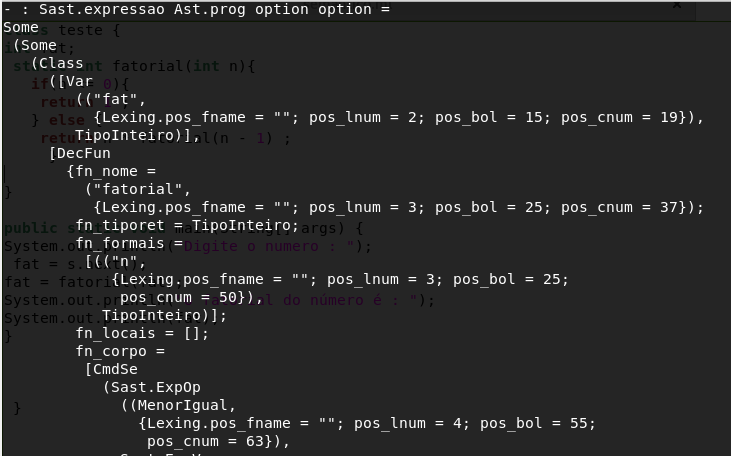
\includegraphics[scale=1]{imagens/printarvsintatica.png}
\end{figure}
\begin{figure}[!ht]
\centering
\caption{Árvore semântica de exemplo.
      \label{fig:6}}
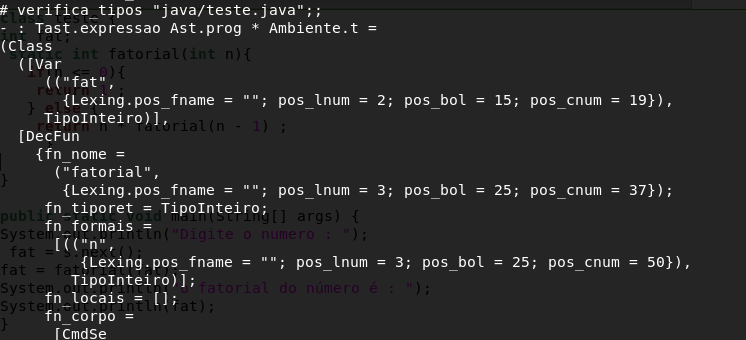
\includegraphics[scale=1]{imagens/arvoretipada.png}
\end{figure}
\begin{figure}[!ht]
\centering
\caption{Exemplo de execução do intérprete.
      \label{fig:7}}
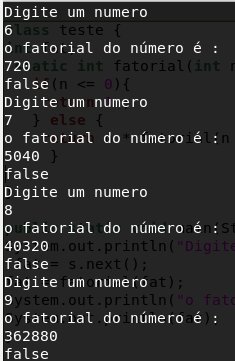
\includegraphics[scale=1]{imagens/interpreteteste.png}
\end{figure}
\clearpage
\addcontentsline{toc}{part}{Apêndice}
\appendix
\section{Bibliografia}
	
%	\begin{thebibliography}
    \begin{enumerate}
	

	\item \href {http://jasmin.sourceforge.net} {\textit   {Documentação e Download do Jasmin}}

	\item \textit {The Java Virtual Machine Specification. Addison Wesley Longman }
	
    	\item \textit {Slides do professor Alexsandro}

	\item \textit { Trabalho de Construção de Compiladores  -  Portugol, Java, JVM [2009] Adair, Andrea, Danilo e Rosângela}

	\end{enumerate}


\end{document} 
